\section {Systemarchitektur}
\author{Benjamin Besic}

\begin{figure}[htp]
    \centering
    \author{David Ignjatovic}
    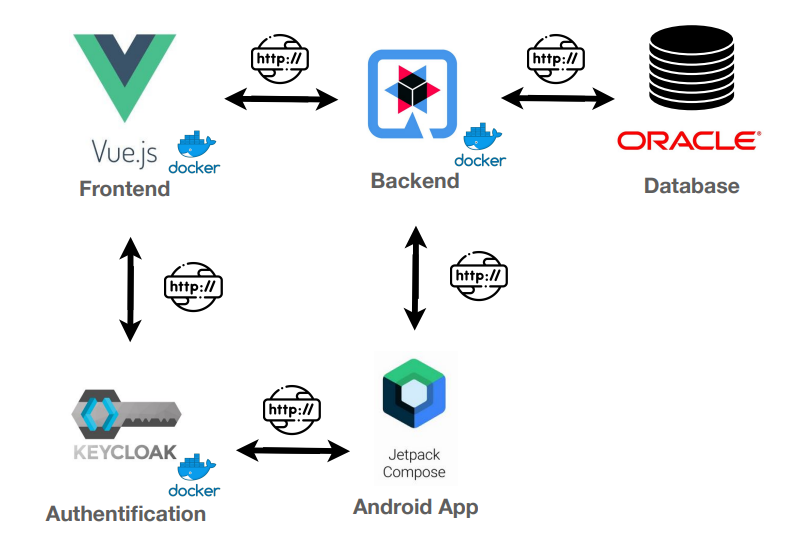
\includegraphics[scale=0.7]{pics/final-sys-arc.PNG}
    \caption{Systemarchitektur des Programms}
    \label{fig:impl:SysArc}
\end{figure}

Der Systemarchitektur kann man entnehmen, dass das Quarkus Backend die zentrale Stelle für alle anderen Technologien bildet.
Das Backend stellt mit Hilfe der Datenbank alle Daten zur Verfügung mittels REST. \\*
Der Keycloak Server sichert die beiden Frontends ab und sorgt dafür, dass keine ungewollten Zugriffe entstehen.
Vue.js benützt dafür ein Keycloak Package, dass eine leichte Integration erlaubt. Die Android App hingegen arbeitet mittels REST Requests mit Keycloak zusammen,
da es zum jetzigen Zeitpunkt keine offizielle Erweiterung für Jetpack Compose gibt.

\subsection{Technologien}

Beim Entwickeln wurden folgende Technologien verwendet:
\begin{itemize}
    \item docker 3.1
    \item Vue.js 2.6.14
    \item quarkus 2.5.0.Final
    \item Jetpack Compose 1.0.1
    \item Keycloak 14.0.0
    \item Java OpenJDK-11
    \item Java EE 8
    \item JBoss Wildfly 7.3.4.GA
\end{itemize}

\section{Datenmodell}
\author{David Ignjatovic}

Ein Datenmodell wird als Darstellung der relevanten Objekte eines Projektes verwendet. 
Unser Datenmodell ist im Großen und Ganzen immer gleichgeblieben. Für den Algorithmus aber haben wir es aber erweitern müssen.

\subsection{Planung}
\author{Benjamin Besic}
Einer der ersten Arbeitsschritte war die Entwicklung eines Datenmodells, welches die Basis der Programmlogik sein soll. Dieses wurde mit einem ERD-Diagramm erstellt.
\begin{figure}[htp]
    \centering
    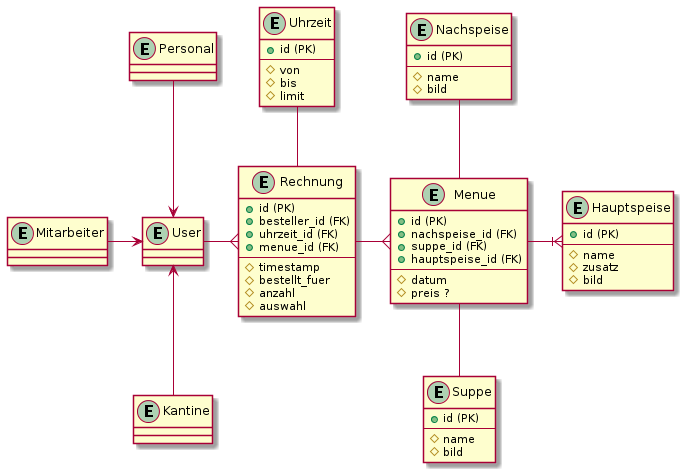
\includegraphics[scale=0.4]{pics/erd-alt.png}
    \caption{Erste Version des Datenmodells}
    \label{fig:impl:ERDold}
\end{figure}

Die erste Version wurde von unserem Team entwickelt, aus den Erfahrungen und Informationen, die wir im Unterricht gesammelt haben. \\*
An dieser Version merkt man, dass die meisten Teile in einzelne Tabellen aufgeteilt wurden. Dies sorgt für Flexibilität und Wiederverwendung von einem Menü, da die einzelnen
Speisen aufgeteilt sind.
Am Anfang war geplant, dass jede Speise auch ein Bild hat, damit der Mitarbeiter weiß, wie die Speise auch wirklich aussieht.\\*
Ebenfalls erkennt man, dass es eine User-Klasse gibt, da Mitarbeiter, Personal und Kantine gleiche Eigenschaften miteinander teilen wie zum Beispiel Vor- und Nachname.\\*


\begin{figure}[htp]
    \centering
    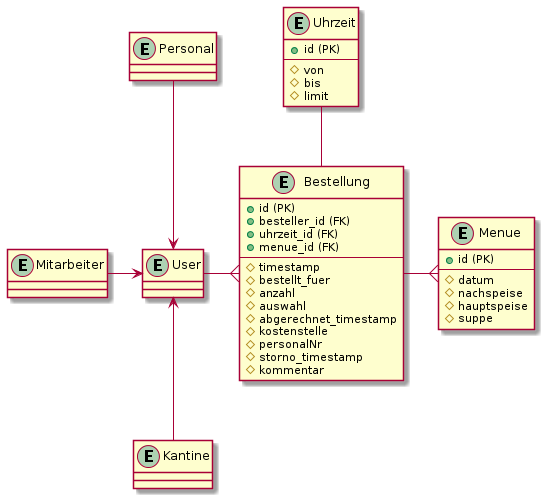
\includegraphics[scale=0.5]{pics/erd-aktuell.png}
    \caption{Finale Version des Datenmodells}
    \label{fig:impl:ERDnew}
\end{figure}

Die finale Version des Datenmodells übernimmt das meiste der ersten Version, jedoch wurde es nach Absprache mit unserer Partnerfirma überarbeitet, um deren Anforderungen mehr zu entsprechen.\\*
Eine wichtige Änderung ist, dass die Menue-Klasse alle Speisen enthält und diese als einfacher Text gespeichert werden. Der Grund dafür ist, dass die Kantine
immer die Menüs händisch eingibt und eine Auswahl von vorhandenen Speisen würde nur den Speicheraufwand unnötig erhöhen. Es kommt eher selten vor, dass die selben Speisen nacheinander kommen.\\*
Was vorher gefehlt hat war der Kommentar und die Möglichkeit die Stornierung eines Menüs nachzuvollziehen. Wenn ein Menü storniert wird, wird es nicht gelöscht, sondern es wird nur 
das Stornodatum gesetzt. Es ist wichtig, dass auch stornierte Bestellungen in der Datenbank bleiben. \\*
Ebenfalls wurde die Abrechnung eines Menüs in der ersten Version nicht berücksichtigt. Die Kosten für das Menü werden dem Mitarbeiter vom Gehalt abgezogen und dies erfolgt anhand 
von den Daten in der Datenbank.


\subsection{Entitäten}
\author{David Ignjatovic}

Eine Entität ist ein bestimmtes Objekt mit den jeweiligen Atributen. Atribute sind die Eigenschaften eins Objektes.
Unser Projektes beinhaltet 5 Entitäten:

\begin{itemize}
  \item Bestellung
  \item Categories
  \item Kantine
  \item Menue
  \item Oeffungszeit
\end{itemize}

\pagebreak

\subsection{Bestellung} 

Die Entität Bestellung enthält die wichtigsten Informationen über einen Mitarbeiter und die dazu ausgewählte Mahlzeit.
Zur Identifikation einer Bestellung verwenden wir eine Id welche generiert wird. \\*

In der Bestellung wird angegebebn von wem die Bestellung bestellt wurde und ob der Mitarbeiter es auch für sich selbst bestellt hat oder für jemand anderen. 
Jeder Mitarbeiter der Firma hat auch eine Personalnummer. Bei jeder Bestellung gibt es die möglichkeit einen Kommentar abzugeben. Dieser wird an die Kantine mitgegeben. Natürlich hat man auch die nöglichkeit 
eine Mahlzeit öfters zu bestellen. Somit hat jeder Mitarbeiter die möglichkeit eine Bestellanzahl mitzugeben. Für das bestellen, bearbeiten aber auch stonieren werden immer die jetztige uhrzeit mitgegeben. \\*

Das wichtigste in der Bestellung ist die Mahlzeit und für wann es bestellt wurde. Dafür verwenden wir die zwei klassen, Oeffnungszeit und Menue. \\*


\definecolor{dkgreen}{rgb}{0,0.6,0}
\definecolor{gray}{rgb}{0.5,0.5,0.5}
\definecolor{mauve}{rgb}{0.58,0,0.82}

\lstset{frame=tb,
  language=Java,
  aboveskip=3mm,
  belowskip=3mm,
  showstringspaces=false,
  columns=flexible,
  basicstyle={\small\ttfamily},
  numbers=none,
  numberstyle=\tiny\color{gray},
  keywordstyle=\color{blue},
  commentstyle=\color{dkgreen},
  stringstyle=\color{mauve},
  breaklines=true,
  breakatwhitespace=true,
  tabsize=3
}

\begin{lstlisting}
    @SequenceGenerator(name = "bestellung_seq_gen", 
                        sequenceName = "BESTELLUNG_SEQ",
                        allocationSize=1)
    @GeneratedValue(strategy = GenerationType.SEQUENCE, 
                        generator = "bestellung_seq_gen")
    @Id
    @Column(name = "BESTELLUNG_ID")
    private Long id;

    @Column(name = "BESTELLTVON",length = 32)
    private String orderedBy;

    @Column(name = "BESTELLTFUER",length = 32)
    private String orderedFor;

    @Column(name = "KOMMENTAR",length = 4000)
    private String comment;

    @Column(name = "PERSONALNUMMER")
    private Long personalNumber;

    @Column(name = "ANZAHL")
    private int menueCounter;

    @Column(name = "STORNIERTUM",length = 6)
    private Timestamp canceledAt;

    @Column(name = "ABGERECHNETUM")
    private Timestamp settledAt;

    @Column(name = "KOSTENSTELLE")
    private Integer moneyPool;

    @Column(name = "ANGELEGTUM",length = 6)
    private Timestamp createdAt;

    @Column(name = "ANGELEGTVON",length = 32)
    private String createdBy;

    @Column(name = "GEAENDERTUM",length = 6)
    private Timestamp changedAt;

    @Column(name = "GEAENDERTVON",length = 32)
    private String changedBy;

    @ManyToOne
    @JoinColumn(name = "OEFFNUNGSZEIT_ID")
    private Oeffnungszeit oeffnungszeit;

    @ManyToOne
    @JoinColumn(name = "MENUE_ID")
    private Menue menue;
\end{lstlisting}

\subsection{Categories}

Die Entität Categories ist ein Enum, welches wir Hauptsächlich für unseren Algorithmus verwenden. Es besteht aus 4 einträgen: \\*


\begin{itemize}
    \item Vegetarisch
    \item Vegan
    \item Schwein
    \item Rind
    \item Huhn
    \item Pute
    \item Salat
    \item Nudel
    \item Süß
    \item Fisch
    \item Sonstiges
\end{itemize}

Die einzelnen Kategorien beschreiben eine Mahlezeit. Sommit kann man ganz einfach zwischen einzelnen Mahlezeiten unterscheiden und sie auch gruppieren.

\subsection{Kantine}

In der Entitäten Kantine befinden sich die wichtigsten Informationen über eine Kantine wie zum Beispiel ob eine Kantine offen ist oder zurzeit geschlossen ist. 
Eine kleine Beschreibung über die Kantine und über das Service ist ebenso enthalten. \\*

\begin{lstlisting}
    @Id
    @Column(name = "KANTINE_ID")
    private Long id;

    @Column(name = "KANTINENBEZEICHNUNG", length = 200)
    private String canteenDesc;

    @Column(name = "SERVICEBEZEICHNUNG", length = 200)
    private String serviceDesc;

    @Column(name = "STATUSKZ", length = 1)
    private char status;

    @Column(name = "ANGELEGTUM",length = 6)
    private Timestamp createdAt;

    @Column(name = "ANGELEGTVON",length = 32)
    private String createdBy;

    @Column(name = "GEAENDERTUM",length = 6)
    private Timestamp changedAt;

    @Column(name = "GEAENDERTVON",length = 32)
    private String changedBy;

\end{lstlisting}

\subsection{Menue}

In der Entität Menue stehen die wichtigsten Informationen über ein Menü. Ein Menü beinhaltet eine Vorspeise, Hauptspeise, Nachspeise und ein Dessert. 
Noch dazu findet man in der Entität ein Datum, um zuzuordnen wann das Menü bestellt wurde. \\*
Neben dem Bestelldatum beinhaltet die Entität Menue auch noch weiter Timestamps.
Die verwendeten Timestamps werden verwendet, um zu speichern, wann ein Menue erstellt wurde oder wann ein Menue geändert wurde. Natürlich wird auch mitgespeichert von wem diese Änderungen durchgeführt wurden. \\*

Die bereits oben genannten Kategorien finden wir in der Entität Menue. 
Diese werden verwendet, um einzelne Menüs zu unterscheiden und mit Hilfe der Kategorien und unserem Algorithmus kann man einfach hervorwagen welche Mahlzeit zu welchem Mitarbeiter am besten passt. \\*

Für jedes Menü wird auch die dazu ausgewählte Kantine mitgespeichert. So weiß man, zu welcher Kantine der Mitarbeiter gehen muss, um sein Menü zu bekommen. \\*

\begin{lstlisting}
    @SequenceGenerator(name = "menue_seq_gen", 
                        sequenceName = "MENUE_SEQ",
                        allocationSize=1)
    @GeneratedValue(strategy = GenerationType.SEQUENCE, 
                    generator = "menue_seq_gen")
    @Id
    @Column(name = "MENUE_ID")
    private Long id;

    @Column(name = "MENUEDATUM")
    private LocalDate date;

    @Column(name = "MENUECODE", length = 1)
    private char code;

    @Column(name = "VORSPEISE", length = 2000)
    private String appetizer;

    @Column(name = "HAUPTSPEISE", length = 2000)
    private String mainDish;

    @Column(name = "NACHSPEISE", length = 2000)
    private String desert;

    @Column(name = "ANGELEGTUM",length = 6)
    private Timestamp createdAt;

    @Column(name = "ANGELEGTVON",length = 32)
    private String createdBy;

    @Column(name = "GEAENDERTUM",length = 6)
    private Timestamp changedAt;

    @Column(name = "GEAENDERTVON",length = 32)
    private String changedBy;

    @Column(name = "CATEGORIES",length = 255)
    private String categories;

    @ManyToOne
    @JoinColumn(name = "KANTINE_ID")
    private Kantine kantine;
\end{lstlisting}

\subsection{Oeffnungszeit}

Die Entitäten Oeffnungszeit zeigt an, ob ein Kantinenraum in Verwendung ist und ob die Maximale Anzahl an Sitzplätzen schon belegt ist. Das Zeitfenster welches beschreibt wann gegessen wird, wird ebenso mitgespeichert. \\*

Um zu wissen welcher Kantinenraum gemeint wird,  wird auch die verwendete Kantine mitgespeichert. \\*

\begin{lstlisting}
    @Id
    @Column(name = "OEFFNUNGSZEIT_ID")
    private Long id;

    @Column(name = "STATUSKZ", length = 1)
    private char status;

    @Column(name = "ZEITFENSTERVON", length = 5)
    private String timeWindowFrom;

    @Column(name = "ZEITFEnSTERBIS", length = 5)
    private String timeWindowTo;

    @Column(name = "MAXPLAETZE", nullable = true)
    private Integer maxPositions;

    @Column(name = "ANGELEGTUM",length = 6)
    private Timestamp createdAt;

    @Column(name = "ANGELEGTVON",length = 32)
    private String createdBy;

    @Column(name = "GEAENDERTUM",length = 6)
    private Timestamp changedAt;

    @Column(name = "GEAENDERTVON",length = 32)
    private String changedBy;

    @ManyToOne
    @JoinColumn(name = "KANTINE_ID")
    private Kantine kantine;
\end{lstlisting}

\section{REST-Schnittstellen}

\colorlet{punct}{red!60!black}
\definecolor{background}{HTML}{EEEEEE}
\definecolor{delim}{RGB}{20,105,176}
\colorlet{numb}{magenta!60!black}

\lstdefinelanguage{json}{
    basicstyle=\normalfont\ttfamily,
    numbers=left,
    numberstyle=\scriptsize,
    stepnumber=1,
    numbersep=8pt,
    showstringspaces=false,
    breaklines=true,
    frame=lines,
    backgroundcolor=\color{background},
    literate=
     *{0}{{{\color{numb}0}}}{1}
      {1}{{{\color{numb}1}}}{1}
      {2}{{{\color{numb}2}}}{1}
      {3}{{{\color{numb}3}}}{1}
      {4}{{{\color{numb}4}}}{1}
      {5}{{{\color{numb}5}}}{1}
      {6}{{{\color{numb}6}}}{1}
      {7}{{{\color{numb}7}}}{1}
      {8}{{{\color{numb}8}}}{1}
      {9}{{{\color{numb}9}}}{1}
      {:}{{{\color{punct}{:}}}}{1}
      {,}{{{\color{punct}{,}}}}{1}
      {\{}{{{\color{delim}{\{}}}}{1}
      {\}}{{{\color{delim}{\}}}}}{1}
      {[}{{{\color{delim}{[}}}}{1}
      {]}{{{\color{delim}{]}}}}{1},
}

\subsection{Allgemein}

In den folgenden Beispielen läuft unser Server lokal auf den Port 8080. Die URL uber die unser
Server erreicht werden kann, ist: http://localhost:8080/menue.

\subsection{Bestellung}

\paragraph{Bestellungen von einem Mitarbeiter}

Um zu sehen welche Bestellungen ein Mitarbeiter gemacht hat, muss der Pfad /bestellung/{username} aufgerufen werden. 
Hierbei handelt es sich um eine GET-Methode die mittels Path parameter die Bestellungen eines bestimmten Mitarbeiters zurück gibt.
Wenn ein Mitarbeiter gefunden wurde und dieser auch mindestens eine Bestellung hat wird der Status 200 zurückgegeben. \\*

Das Reslutat für den Mitarbeiter spabo sieht folgendermassen aus:


URL: GET \colorbox{white}{\lstinline[basicstyle=\ttfamily\color{black},language=html]| http://localhost:8080/menue/bestellung/spabo|}


Output:

\begin{lstlisting}[language=json,firstnumber=1]
{
    "createdAt": "2021-11-26T15:33:33.62898Z[UTC]",
    "id": 1315,
    "menueDate": "2021-11-29",
    "menueName": "Spaghetti",
    "orderedFor": "spabo",
    "timeWindow": "11:15 - 11:45"
}
\end{lstlisting}

Die Bestellungen wird nach dem Datum, an dem eine Bestellungen angelegt wurde, sortiert. Somit werden immer die neusten Bestellungen gleich am Anfgang angezeigt.

\paragraph{Anzahl der Bestellungen pro Wochentag eines Mitarbeitern}

Wenn man sehen will wie oft ein Mitarbeiter pro Wochentag ein Menue bestellt hat, muss der Pfad /bestellung/stats/{username} aufgerufen werden.
Es werden alle Wochentage angezeigt an denen ein Mitarbeiter eine bestellung getätigt hat. Wenn mindestens ein Wochentag mit einer bestellung zur verfügung steht, wird der Status 200 zurückgegeben.

Das Reslutat für den Mitarbeiter besbe sieht folgendermassen aus:


URL: GET \colorbox{white}{\lstinline[basicstyle=\ttfamily\color{black},language=html]|http://localhost:8080/menue/bestellung/stats/besbe|}


Output:

\begin{lstlisting}[language=json,firstnumber=1]
[
    {
    "amount": 2,
    "weekday": "Montag"
    },
    {
    "amount": 1,
    "weekday": "Mittwoch"
    },
    {
    "amount": 1,
    "weekday": "Donnerstag"
    },
    {
    "amount": 0,
    "weekday": "Dienstag"
    }
]
\end{lstlisting}

\paragraph{Alle Kategorien}

Damit man alle Kategorien sieht, welche eine Mahlzeit haben kann, muss der Pfad bestellung/categories aufgerufen werden.
Wichtig ist es, dass man hier keinen namen als Parameter übergibt. \\*

Anhand der Kategrien, wird mit hilfe eines Algorithmus enschieden, welche Mahlzeit am besten zu einem Mitarbeiter passt. 

Die verwendbaren Kategorien sehen folgendermassen aus:

URL: GET \colorbox{white}{\lstinline[basicstyle=\ttfamily\color{black},language=html]|http://localhost:8080/menue/bestellung/categories|}

Output:

\begin{lstlisting}[language=json,firstnumber=1]
[
    "Vegetarisch",
    "Vegan",
    "Schwein",
    "Rind",
    "Huhn",
    "Pute",
    "Salat",
    "Nudel"
    "Fisch",
    "Sonstiges"
]
\end{lstlisting}

\paragraph{Alle Kategorien von einem bestimmten Mitarbeiter}

Um zu sehen welche Kategorien ein Mitarbeiter bestellt hat, muss der Pfad /bestellung/categories/{username} aufgerufen werden.

Wenn ein User keine Bestellungen getätigt hast, werden auch keine Kategorien zurückgegeben. In dem folgenden Beispiel kann man aber sehen, wie das Reslutat
für den Mitarbeiter spabo aussieht:

URL: GET \colorbox{white}{\lstinline[basicstyle=\ttfamily\color{black},language=html]|http://localhost:8080/menue/bestellung/categories/spabo|}

Output:

\begin{lstlisting}[language=json,firstnumber=1]
[
    "Vegetarisch",
    "Nudel",
    "Vegan",
    "Schwein",
    "Salat",
    "Pute"
]
\end{lstlisting}


\paragraph{Alle Bestellungen an einem bestimmten Tag}

Damit die Kantine sehen kann, welche Bestellungen an welchen Tagen zugewissen worden sind, muss der Pfad /bestellung?date=datum aufgerufen werden.

Es kann aber auch sein, das es an bestimmten Tagen keine bestellungen gibt. Deshalb werden auch keine Ergebnisse zurückgegeben.

Um aber zu veranschaulichen, wie manche Bestellungen an einem bestimmten Zeitpunkt zurückgegeben werden, verwenden wir das den 16.03.2022.

URL: GET \colorbox{white}{\lstinline[basicstyle=\ttfamily\color{black},language=html]|http://localhost:8080/menue/bestellung?date=2022-03-16|}

Output:

\begin{lstlisting}[language=json,firstnumber=1]
[
    {
        "code": "A",
        "date": "2022-03-16",
        "menue": "Schnitzel",
        "menueCounter": 1,
        "orderedFor": "spabo",
        "personalNumber": 1023,
        "timewindow": "11:15 - 11:45"
    },
    {
        "code": "C",
        "date": "2022-03-16",
        "menue": "Eisbergsalat",
        "menueCounter": 1,
        "orderedFor": "spabo",
        "personalNumber": 1023,
        "timewindow": "12:00 - 12:30"
    },
    ...
    ]
\end{lstlisting}


\paragraph{Bestellung erstellen}

WIP


\paragraph{Bestellung stornieren}

WIP

\subsection{Menue}

\paragraph{Alle Menüs}

Um sehen zu können, welche Menüs es überhapt schon gab, muss der Pfad /menues aufgerufen werden. 

Ein Beispiel für ein Menue sieht folgendermassen aus:

URL: GET \colorbox{white}{\lstinline[basicstyle=\ttfamily\color{black},language=html]|http://localhost:8080/menue/menues|}


\begin{lstlisting}[language=json,firstnumber=1]
[
    {
        "appetizer": "Suppe",
        "categories": "Vegan;Vegetarisch;Salat",
        "code": "C",
        "date": "2022-03-22",
        "dessert": "Milka",
        "id": 706,
        "mainDish": "Kartofell Salat"
    },
    {
        "appetizer": "Suppe",
        "categories": "Vegan;Vegetarisch;Salat",
        "code": "C",
        "date": "2022-03-22",
        "dessert": "Milka",
        "id": 705,
        "mainDish": "Kartofell Salat"
    },
    ...
]
\end{lstlisting}

\paragraph{Menü erstellen}

Damit die Kantine ein Menü erstellen kann, wird ein POST-Request an den Pfad PFAD ÄNDERN geschickt.

Da eine Bestellung aus genau 3 Menues besteht, werden auch 3 POST-Requests abgeschickt. Die werte werden in Form eines JSON Objekt abgeschickt.

Ein Beispiel für eine Bestellung sieht folgendermassen aus:

URL: POST \colorbox{white}{\lstinline[basicstyle=\ttfamily\color{black},language=html]|http://localhost:8080/menue/...|}


JSON Objekt für Menue A:

\begin{lstlisting}[language=json,firstnumber=1]
{
    "id":null,
    "date":"2022-03-22",
    "code":"A",
    "appetizer":"Suppe",
    "mainDish":"Pasta",
    "dessert":"Milka",
    "categories":"Rind;Nudel"
}
\end{lstlisting}

JSON Objekt für Menue B:

\begin{lstlisting}[language=json,firstnumber=1]
{
    "id":null,
    "date":"2022-03-22",
    "code":"B",
    "appetizer":"Suppe",
    "mainDish":"Lachs",
    "dessert":"Milka",
    "categories":"Fisch"
}
\end{lstlisting}

JSON Objekt für Menue C:

\begin{lstlisting}[language=json,firstnumber=1]
{
    "id":null,
    "date":"2022-03-22",
    "code":"C",
    "appetizer":"Suppe",
    "mainDish":"Kartofell Salat",
    "dessert":"Milka",
    "categories":"Vegan;Vegetarisch;Salat"
}
\end{lstlisting}

Wie man sehen kann, werden die Kategorien in einem String übergeben. Die Kategorien werden aber dann in getrennt und als Enum gespeichert.

\paragraph{Menü verändern}

\paragraph{Menü-Vorschlag (Recomendation)}

\paragraph{Alle Menüs an einem bestimmten Tag}


\subsection{Oeffnungszeiten}

\paragraph{Alle Aktiven Essenszeiten}

\paragraph{Freien Tische}


\section{Authentifizierung}

\section {Interface Webapp}
\author{Benjamin Besic}
\subsection{Planung}

Nachdem das Datenmodell feststand wurden UI-Prototypen entwickelt, die das Aussehen der Vue-App darstellen sollen.

\begin{figure}[htp]
    \author{Benjamin Besic}
    \centering
    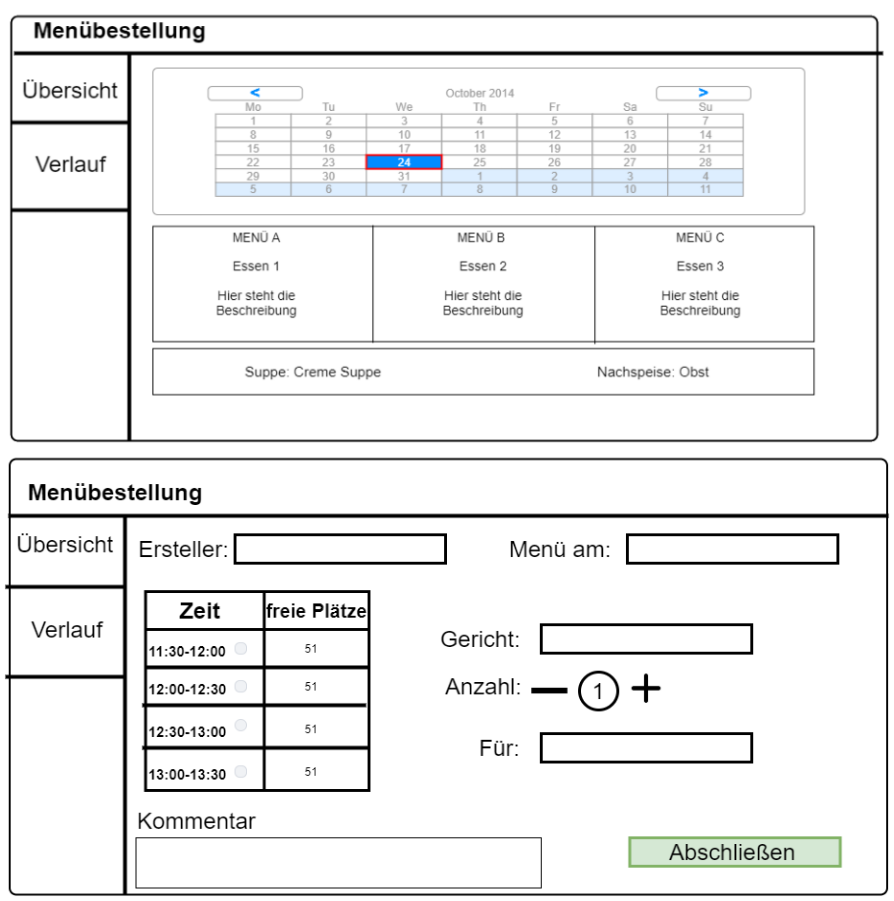
\includegraphics[scale=0.3]{pics/UI-Bestellung-Prototyp.png}
    \caption{UI-Prototypen für den Bestellvorgang}
    \label{fig:impl:UIPlanningBest}
\end{figure}

\subsubsection{Bestellvorgang}
Beim Entwickeln stehen die Benutzerfreundlichkeit und das Aussehen auf mobilen Geräten an erster Stelle. Anhand dessen ist die Navigationsleiste am Wichtigsten.
Diese soll den Benutzer auf alle Sichten führen können und dem Benutzer ermöglichen, sich auszuloggen. \\*
Der Kalender muss übersichtlich sein und die Tage, an denen Bestellungen nicht möglich sind, sollten ausgeblendet sein. Ebenfalls soll auch in die Vergangenheit geschaut werden können.\\*
Um den Rest des Platzes auszunutzen wurde eine Menüauswahlt geplant, die soviel wie möglich Information darstellen kann, ohne den Benutzer zu überfordern.
Nach langem Überlegen wurden die drei Menüs groß als Kästen dargestellt, um soviel wie möglich innerhalb dieser darstellen zu können.
Die Vor- und Nachspeise ist kleiner dargestellt, da man keine Entscheidung darüber machen kann.\\*
Die Sicht nachdem man sich ein Menü ausgewählt hat, soll so kompakt wie möglich sein, da auch die mobile Ansicht ohne Probleme nutzbar sein soll.
Alle Informationen, die vom Benutzer eingegeben werden müssen, sollen in der Form eines Formulars angezeigt werden und andere Informationen wie Ersteller und Gericht 
werden automatisch eingesetzt.
\begin{figure}[htp]
    \author{Benjamin Besic}
    \centering
    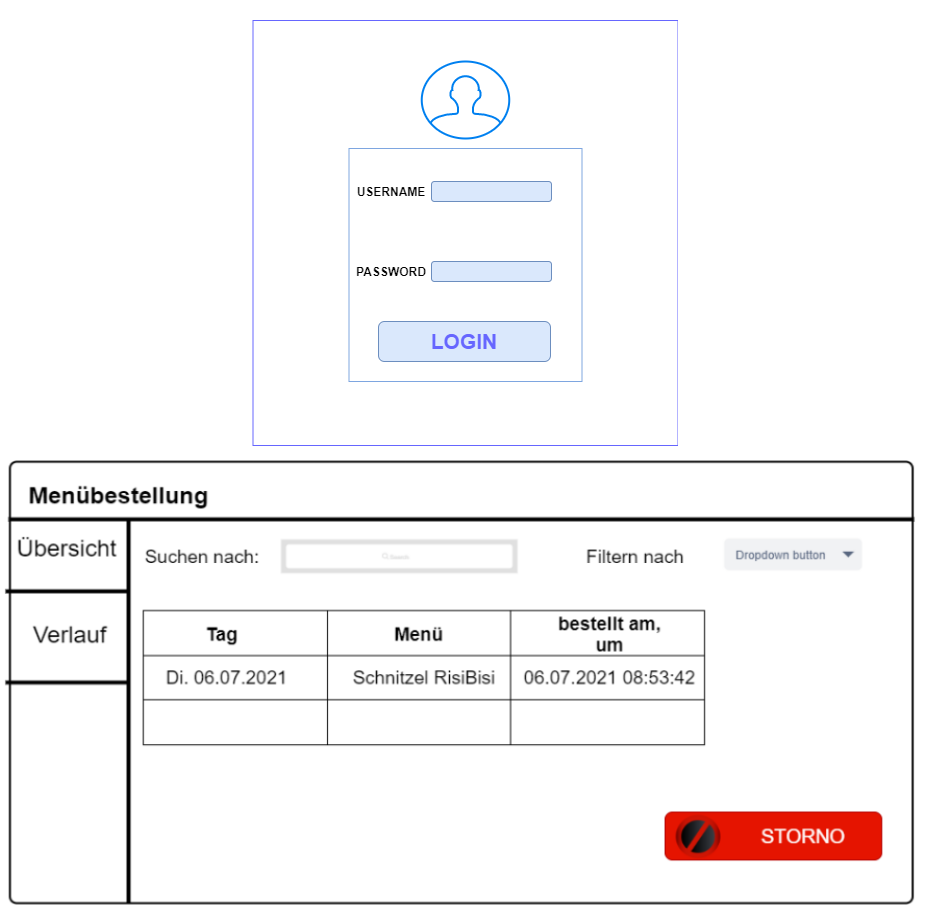
\includegraphics[scale=0.36]{pics/UI-Login-Uebersicht-Prototyp.png}
    \caption{UI-Prototypen für den den Login und die Übersicht}
    \label{fig:impl:UIPlanningLogUebersicht}
\end{figure}

\subsubsection{Login und Übersicht}
Der Login soll einladend sein, hat aber keinen besonderen Anforderungen zu entsprechen \\*
Die Übersicht über die bereits bestellten Menüs soll dem Benutzer alle wichtigen Informationen auf einen Blick geben.
Das Stornieren soll ebenfalls simpel gehalten werden, damit der Benutzer nicht darüber nachdenken muss.
Der Benutzer soll auch eine Möglichkeit haben die Bestellungen zu filtern, um bestimmte Zeitpunkte bzw. Menüs einfacher zu finden.


\subsection{Login}
Beim Aufrufen der Webapp wird man zunächst zu der Login-Seite weitergeleitet. Wie diese fungiert, sieht man in der nächsten Abbildung. \\*
Der Login dient in erster Hinsicht dazu, um festzustellen ob der Benutzer ein Mitarbeiter oder Kantinenmitarbeiter ist.
Denn nach dem Login wird man entweder zur Mitarbeiter-Ansicht oder Kantinenmitarbeiter-Ansicht weitergeleitet. \\*

\begin{figure}[htp]
    \centering
    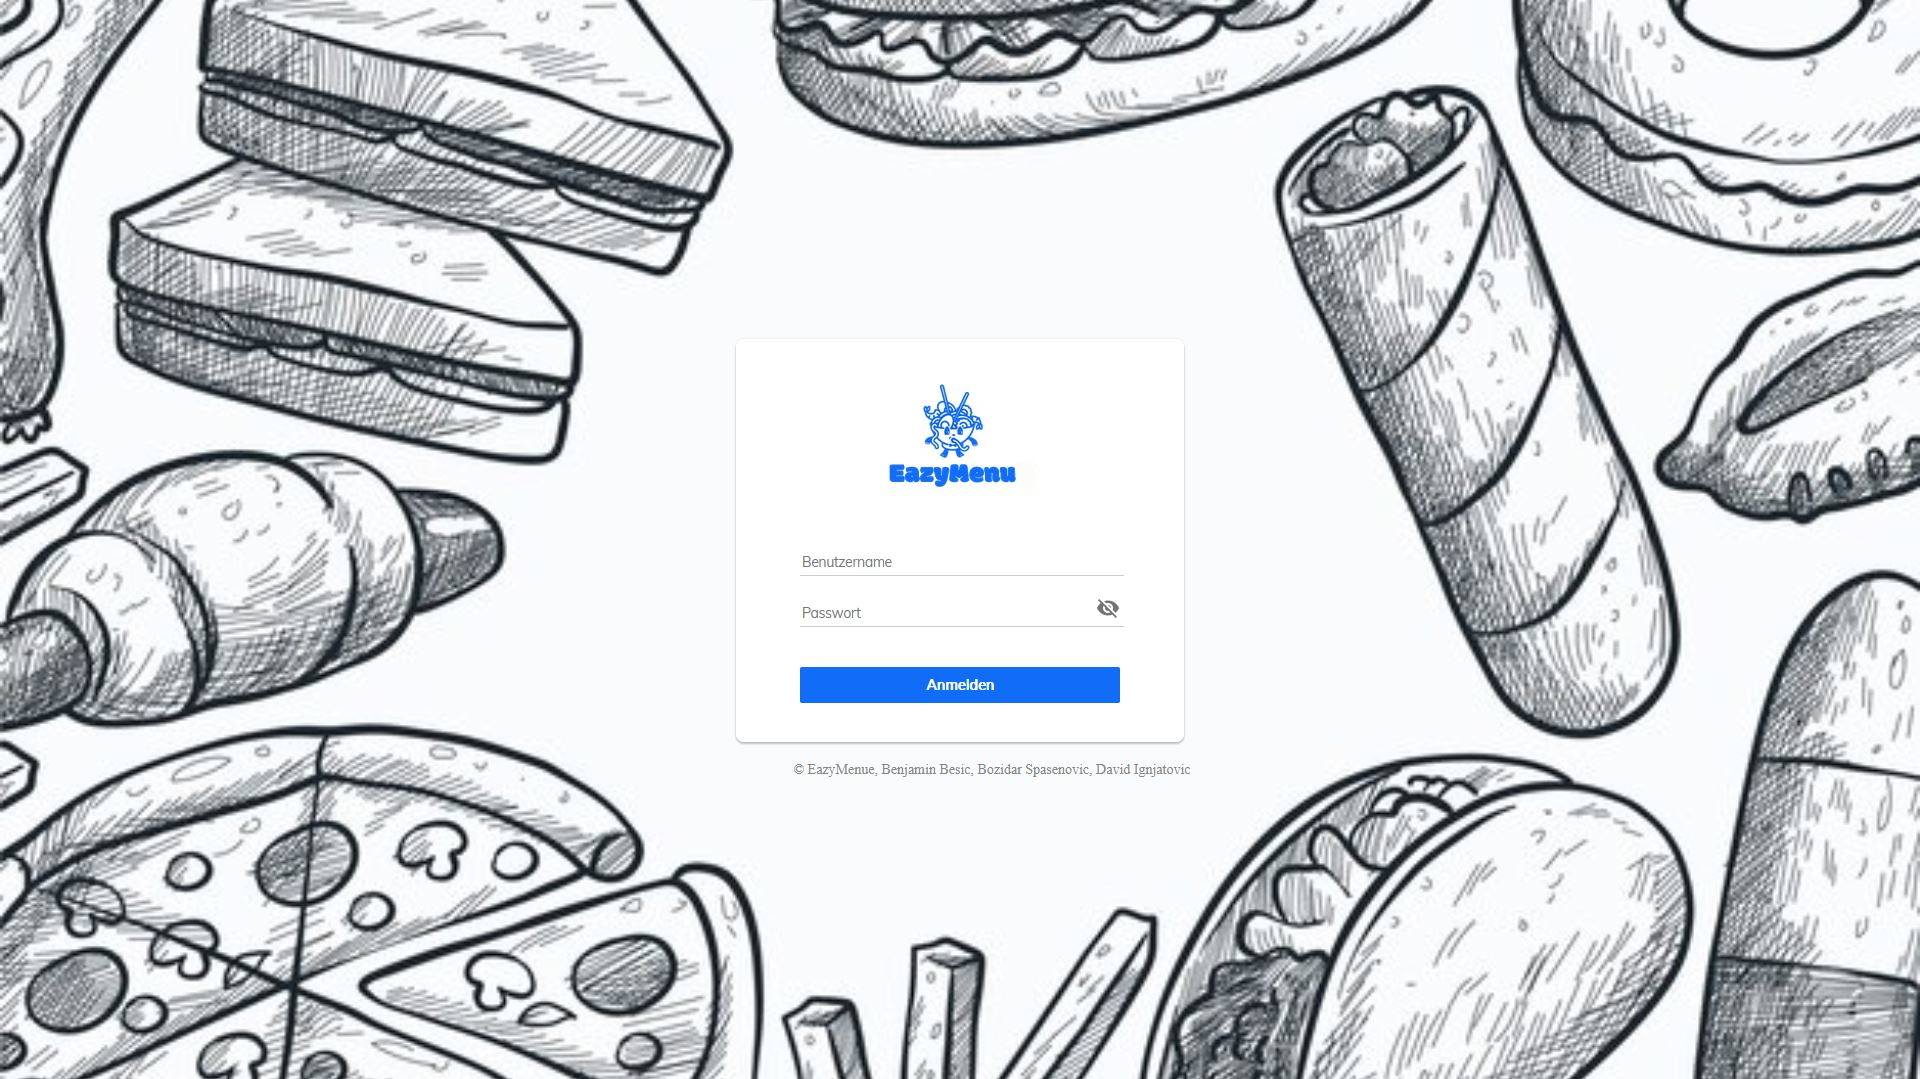
\includegraphics[scale=0.3]{pics/login_screen_vue.JPG}
    \caption{Login Screen}
    \label{fig:impl:LoginVue}
\end{figure}


\pagebreak

\subsection {Mitarbeiter-Ansicht}

\subsubsection {Home}
\label{sec:MitHome}
Das Erste, was ein Mitarbeiter zu sehen bekommt, ist die Home Ansicht. In dieser Ansicht ist eine Kalender und die Menüauswahl enthalten. \\*
Der Benutzer kann im Kalender das gewünschte Bestelldatum anklicken, dadurch wird automatisch die Menüauswahl aktualisiert. Man kann sich in die Zukunft, sowohl auch 
in die Vergangenheit klicken, um sich Auskunft über die vergangenen/kommenden Menüs zu beschaffen. Die Ansicht ist nur auf die Bestelltage beschränkt, an denen Menüs angeboten werden.\\*
Nach der erfolgreichen Datumswahl hat man unten drei Menüs zur Auswahl, sowohl wie die dazugehörige Vor- und Nachspeise. Das dem Benutzer empfohlene Menü (Analyse aus seinem Bestellverlauf) wird grün hinterlegt.
Neben den Bestellköpfen befindet sich ein Fragezeichen-Knopf, wenn man über diesen geht werden einem die Kategorien des Menüs angezeigt.
\\* Wenn die Bedingungen für eine Bestellung erfüllt sind,
kann man auf einen der drei Bestellknöpfe drücken, um zur Bestellansicht weitergeleitet zu werden. Sind diese Bedingungen nicht erfüllt, sind die Knöpfe ausgeschaltet. \\*
Weiters werden unter den Menüs noch relevante Informationen angezeigt. Durch das Klicken des Fragezeichen-Knopfs wird ein Bild der 14 Allergene geöffnet.

\begin{figure}[htp]
    \centering
    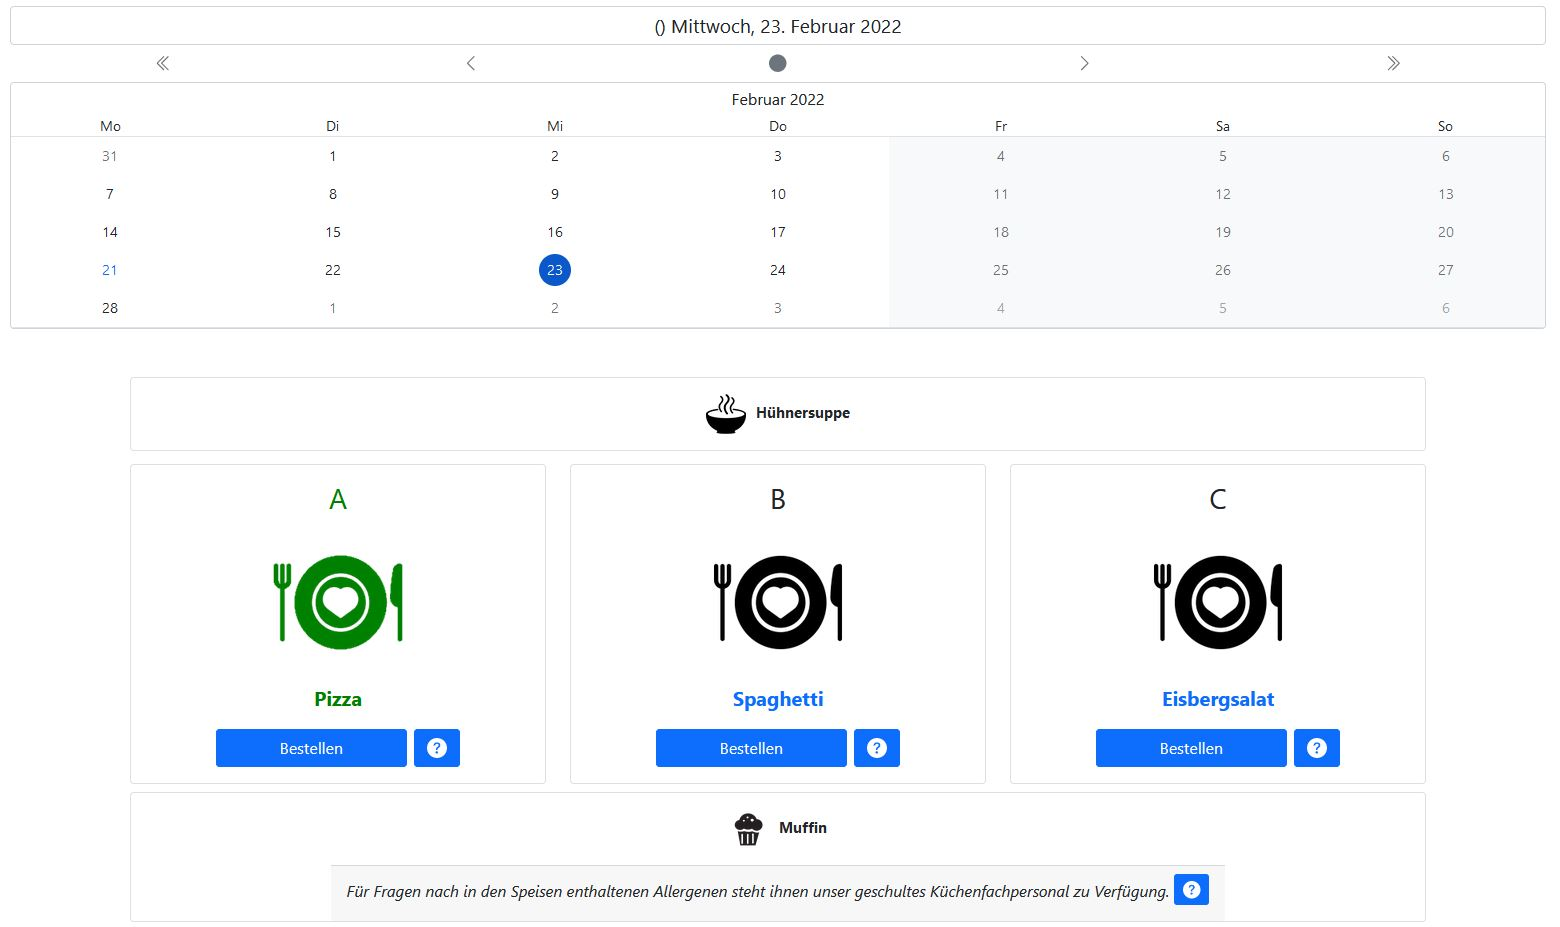
\includegraphics[scale=0.35]{pics/mitarbeiter-home.JPG}
    \caption{Home Ansicht eines Mitarbeiters}
    \label{fig:impl:HomeMitarbeiter}
\end{figure}

\begin{figure}[htp]
    \centering
    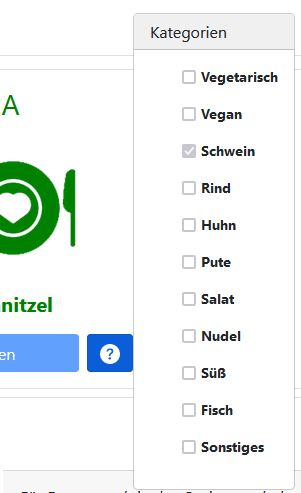
\includegraphics[scale=0.5]{pics/kategorien_mitarbeiter.JPG}
    \caption{Kategorieanzeige eines Menüs}
    \label{fig:impl:CategoriesForMenue}
\end{figure}

\pagebreak

\subsubsection {Bestellansicht}

In der Bestellansicht werden die nötigen Daten für die Bestellung ausgefüllt. Die ersten drei Felder sind automatisch ausgefüllt, aufgrund der vorherigen Auswahl. \\*
Die Tabelle auf der rechten Seite enthält alle Bestellzeiträume, die es gibt. Man kann nur eine gleichzeitig auswählen. Außerdem stehen die freien Plätze dabei, die aus der Datenbank geladen werden.\\*
Die Anzahl der Menüs kann durchs Klicken des Plus- und Minusknopfs angepasst werden.  \\*
Darunter steht voreingestellt der Benutzer, doch dies kann verändert werden, um das Menü für einen anderen Mitarbeiter bestellen zu können. \\*
Abschließend kann man noch einen Kommentar an die Kantine mitgeben, falls es etwaige Extrawünsche geben sollte. \\*
Die Bestellung kann durch den Abschließen-Knopf durchgeführt werden und Abbrechen kann man jederzeit mit dem Abbrechen-Knopf.
Die Bestellung ist erst ausführbar, sobald alle Felder außer des Kommentars ausgefüllt wurden.
\begin{figure}[htp]
    \centering
    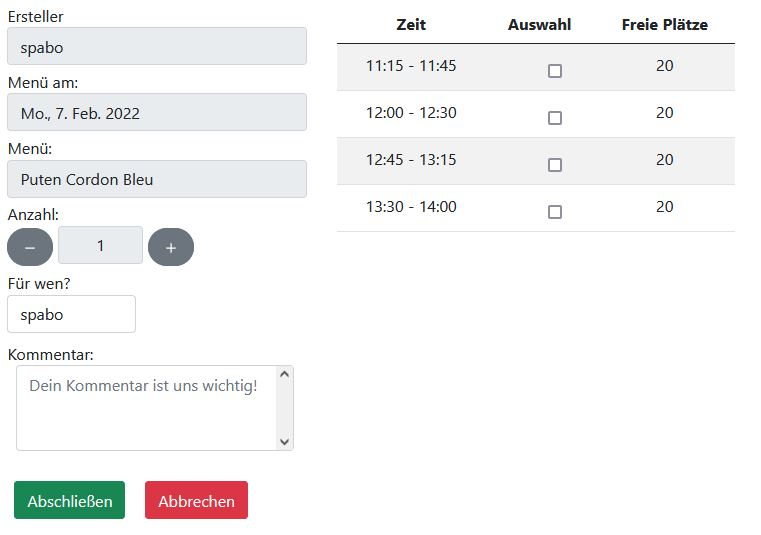
\includegraphics[scale=0.7]{pics/mitarbeiter-bestellen.JPG}
    \caption{Bestellansicht}
    \label{fig:impl:BestellenMitarbeiter}
\end{figure}
\pagebreak

\subsubsection {Bestellübersicht}

Die Bestellübersicht dient dem Benutzer dazu seine Bestellhistorie nachzuvollziehen. Zu jeder Bestellung ist der Name des bestellten Menüs, das Menüdatum, der Bestellzeitpunkt und die Essenszeit zugeordnet. \\*
Der Benutzer hat die Möglichkeit, oben in der Suchleiste, die Bestellungen nach Name oder Menüdatum zu filtern. Das Filtern erfolgt direkt nach der Eingabe. \\*
Man kann jede Bestellung anklicken und falls eine Bestellung die Stornierbedingungen erfüllt kann diese mit dem unten gelegen Storno-Button storniert werden.
Nach einer erfolgreichen Stornierung verschwindet die Bestellung aus dem Verlauf, doch in der Datenbank wird nur das Stornierdatum gesetzt und somit wird die Bestellung ungültig gemacht. 


\begin{figure}[htp]
    \centering
    \includegraphics[scale=0.3]{pics/mitarbeiter-bestellen-übersicht.JPG}
    \caption{Bestellungsübersicht}
    \label{fig:impl:BestellenMitarbeiterUebersicht}
\end{figure}
\pagebreak

\subsubsection {Statistiken}

Der Benutzer kann in dieser Ansicht mehr Informationen über seine vergangenen Bestellungen bekommen.
Durch das Wechseln des Tabs oben links wird entweder eine Statistik über die Kategorien oder über die Wochentage angezeigt. \\*
Die Informationen der Statistiken beziehen sich auf alle Bestellungen, die der Nutzer bereits getätigt hat.

\begin{figure}[htp]
    \centering
    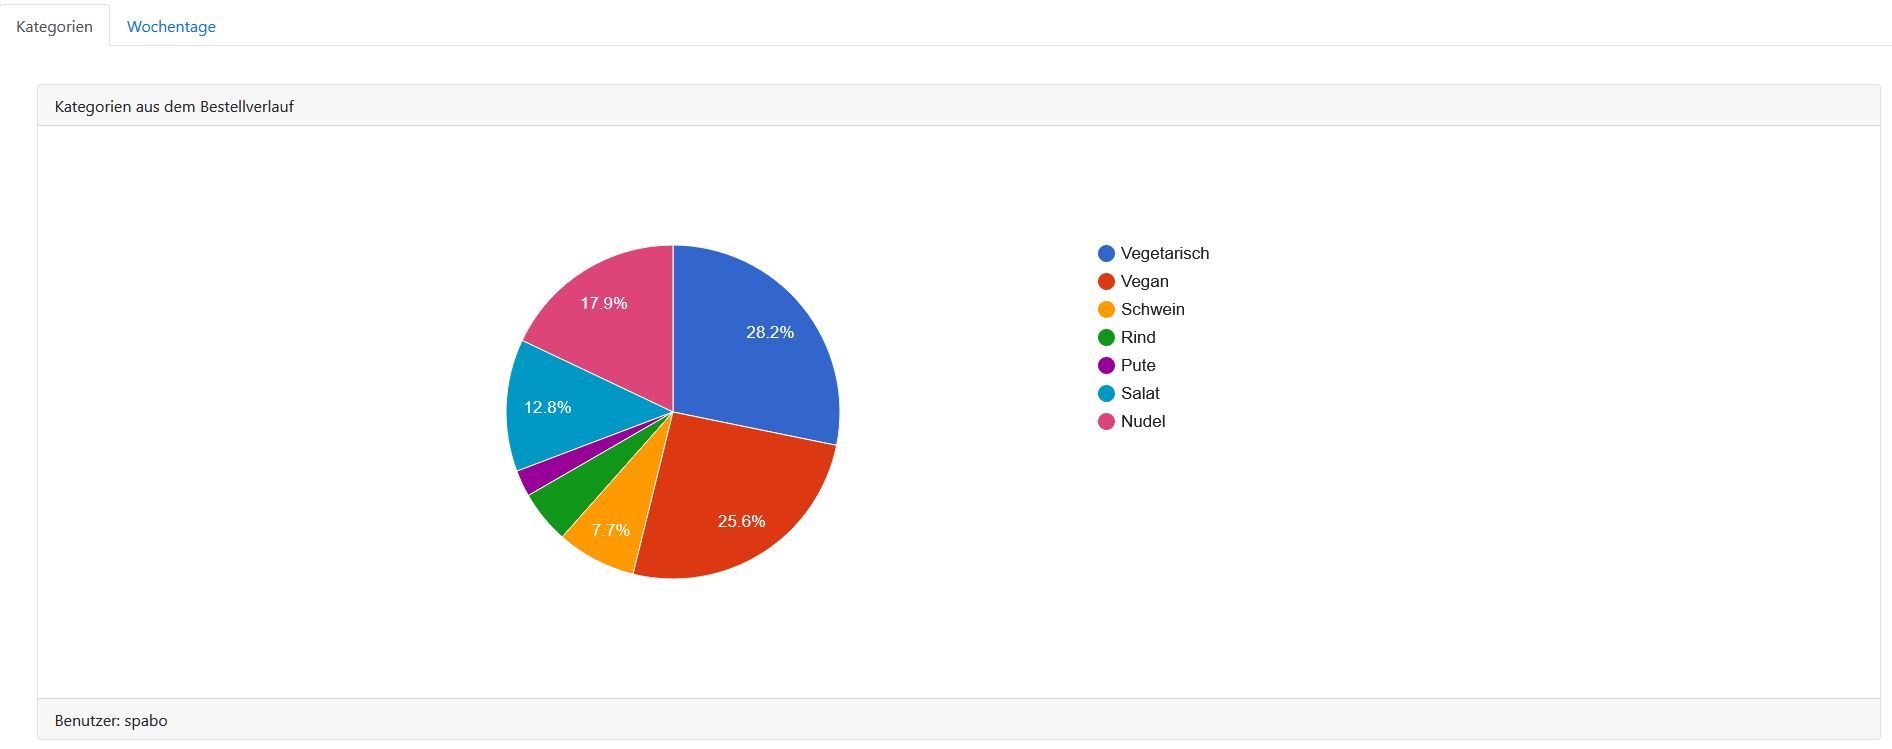
\includegraphics[scale=0.3]{pics/statistiken_kategorien.JPG}
    \caption{Kategorie Statistiken}
    \label{fig:impl:StatsCategories}
\end{figure}

\begin{figure}[htp]
    \centering
    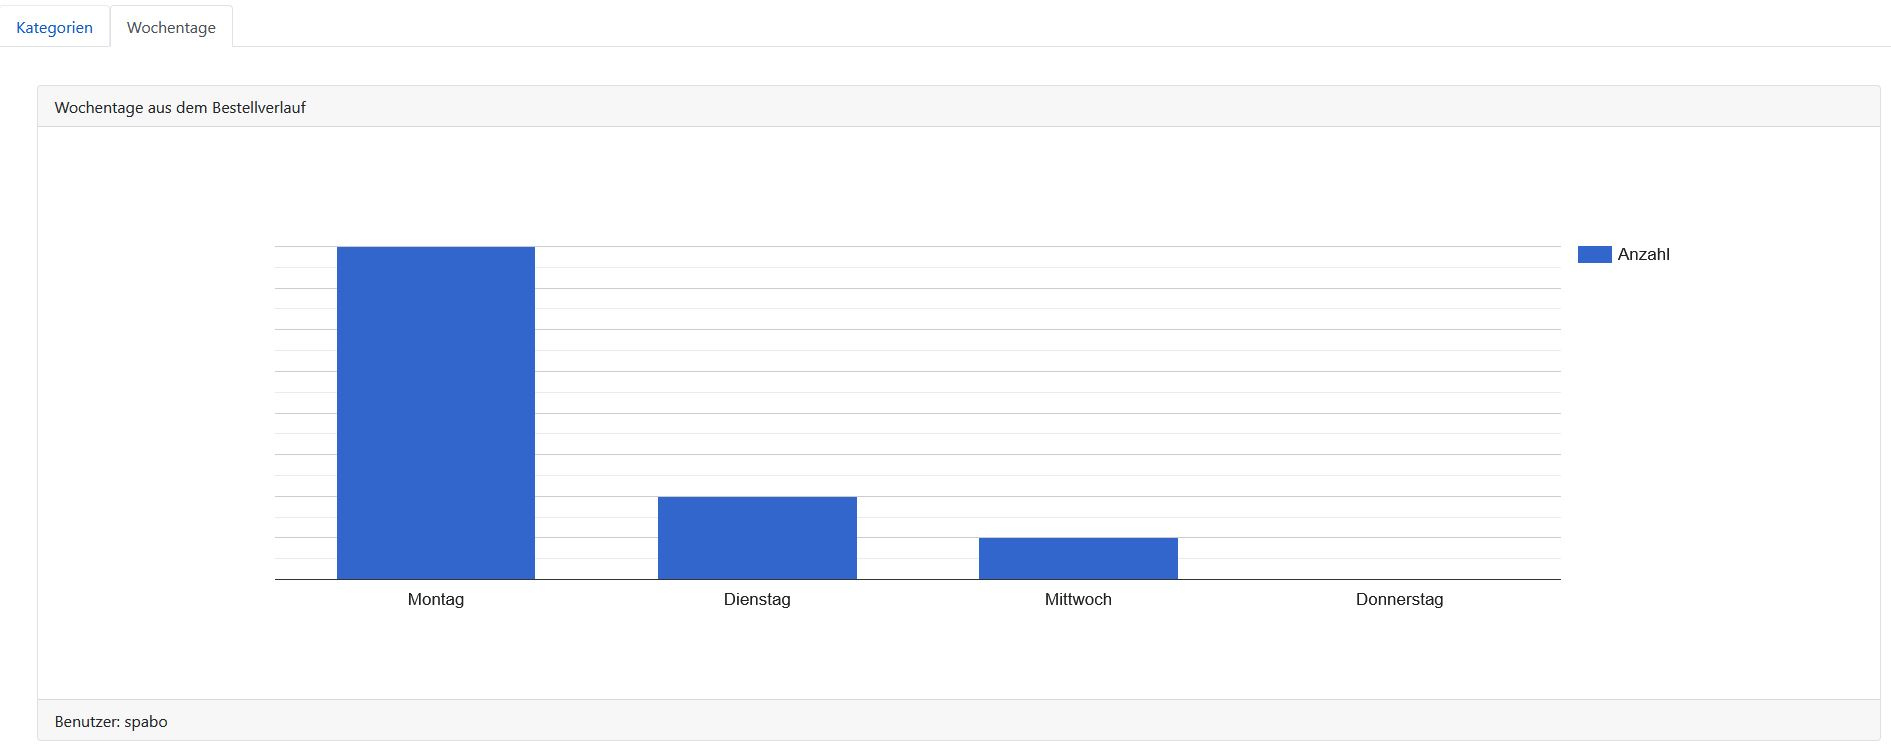
\includegraphics[scale=0.3]{pics/statistiken_wochentage.JPG}
    \caption{Wochentage Statistiken}
    \label{fig:impl:WeekDaysCategories}
\end{figure}

\pagebreak

\subsection {Kantinen-Ansicht}
\subsubsection {Home}

Die Startseite der Kantinenmitarbeiter ähnelt der Ansicht der Mitarbeiter. \hyperref[sec:MitHome]{Siehe hier}. \\*
Die Unterschiede sind, dass die Kantine Textfelder für jedes Menü und dessen Vor- und Nachspeise hat.
Ebenfalls erscheint beim Kategorien-Knopf eine Liste von Kategorien zum Anhaken, um dem Menü die entsprechenden Kategorien zuzuordnen. \\*
Die Textfelder und Kategorien können bearbeitet werden, um ein vorhandenes Menü zu aktualisieren oder um ein neues zu erstellen.
Die Erstellung bzw. die Änderung kann durch den Speichern-Knopf durchgeführt werden. Je nach Fall werden neue Menüs an das Backend geschickt oder ein
vorhandenes wird aktualisiert.

\begin{figure}[htp]
    \centering
    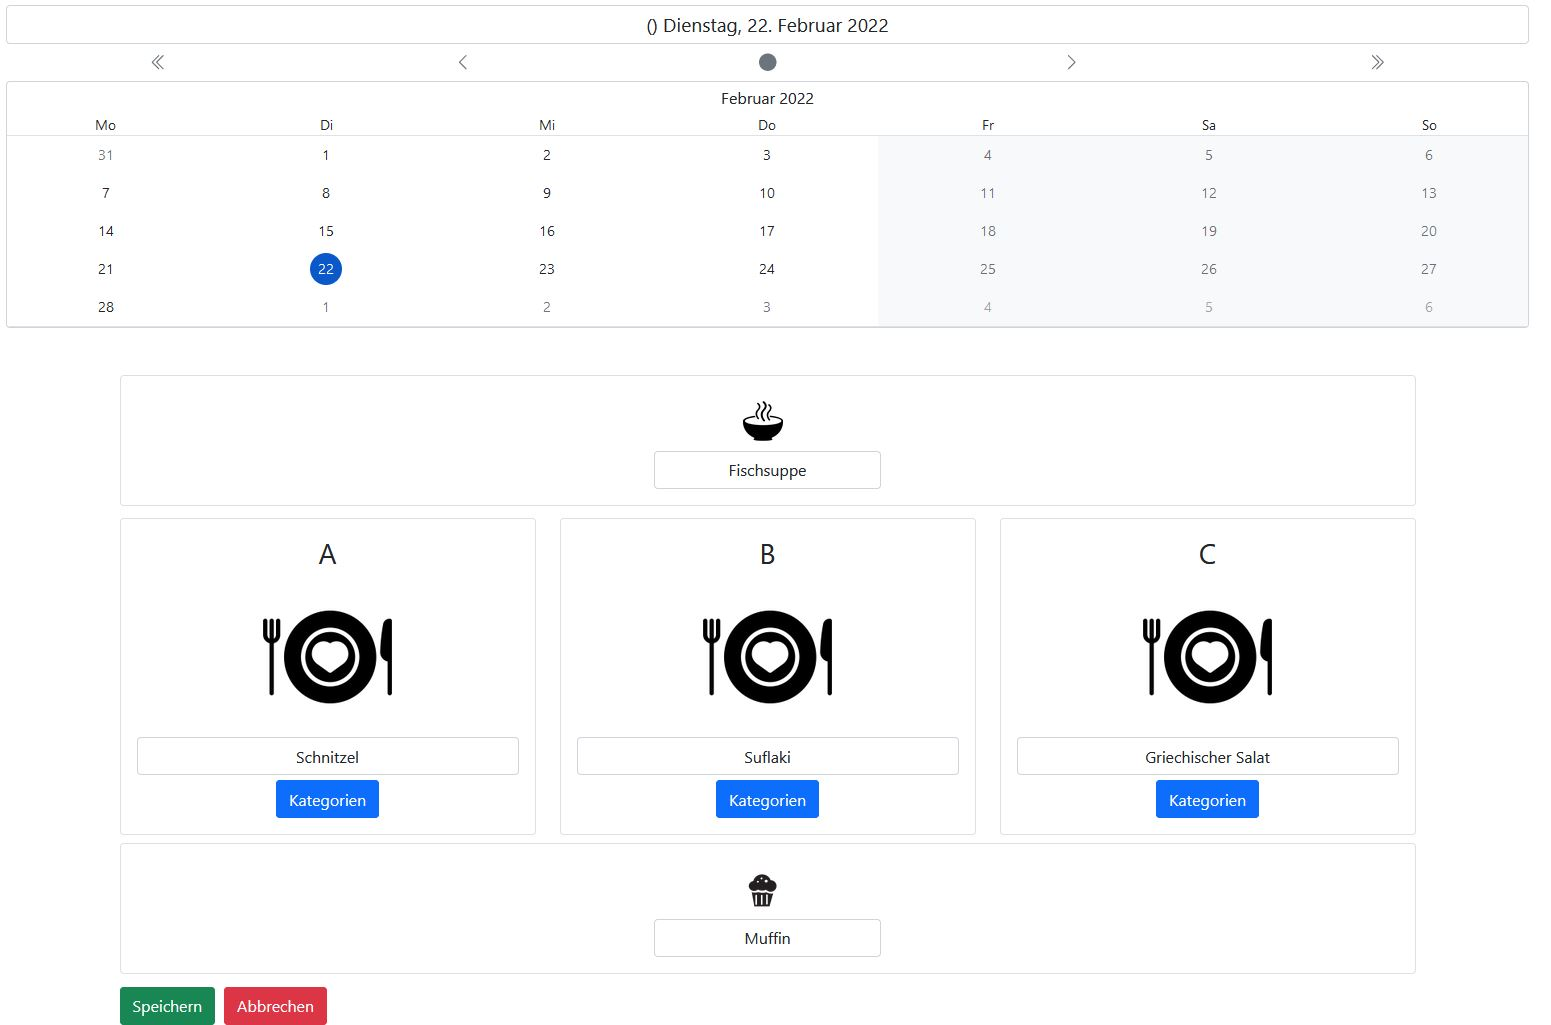
\includegraphics[scale=0.35]{pics/kantine_home.JPG}
    \caption{Kantine Homeansicht}
    \label{fig:impl:CantineHome}
\end{figure}

\begin{figure}[htp]
    \centering
    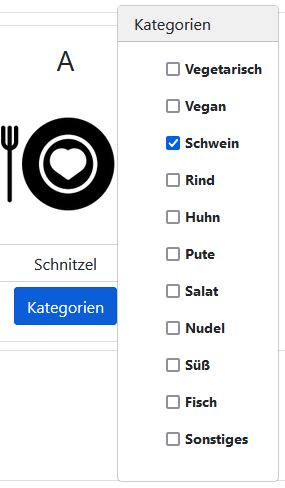
\includegraphics[scale=0.4]{pics/kategorien_kantine.JPG}
    \caption{Kategorieauswahl}
    \label{fig:impl:CategoryChooseCantine}
\end{figure}
\pagebreak

\subsubsection {Drucken}

Die Druckansicht dient den Kantinenmitarbeitern dazu, um die Bestellungen des jeweiligen Tages auch durchführen zu können.
Der Tag kann durch eine Datumsauswahl bestimmt werden.
Die Ansicht zeigt alle nötigen Informationen, damit die Kantine einen Überblick über die Bestellungen hat und dementsprechend das Essen vorbereiten kann.
Es sind die Essenszeiten sowie Anzahl der jeweiligen Menücodes summiert für einen schnellen Überblick. \\*
Durch das Drücken des Drucken-Knopfs hat die Kantine die Möglichkeit ein pdf-Dokument aus der kompletten Ansicht, die unter dem Knopf zu sehen ist, zu drucken.
Dies dient dazu, dass sie einen Ausdruck auf Papier haben, der für die Kantine praktischer ist.

\begin{figure}[htp]
    \centering
    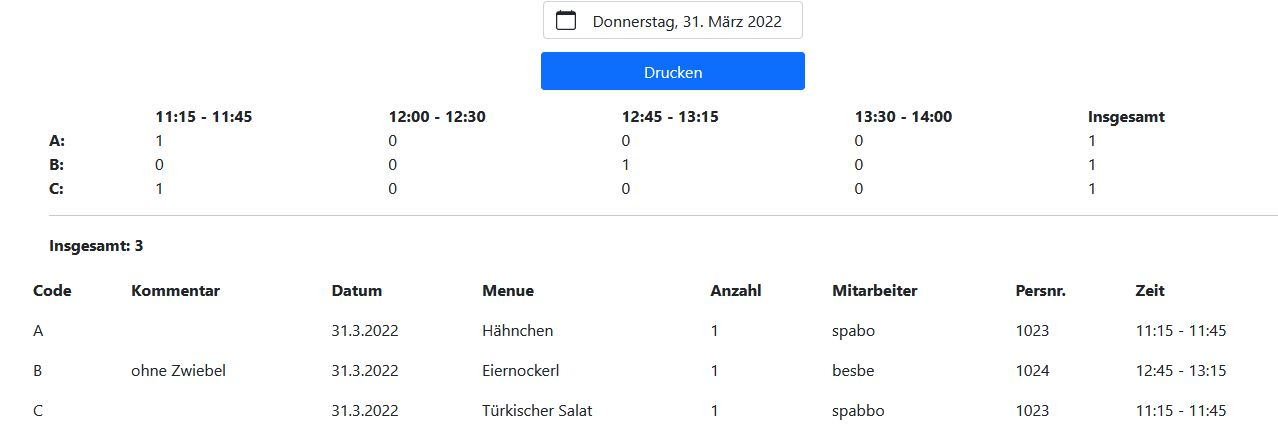
\includegraphics[scale=0.45]{pics/kantine_drucken.JPG}
    \caption{Druckansicht der Kantine}
    \label{fig:impl:CantinePrint}
\end{figure}

\begin{figure}[htp]
    \centering
    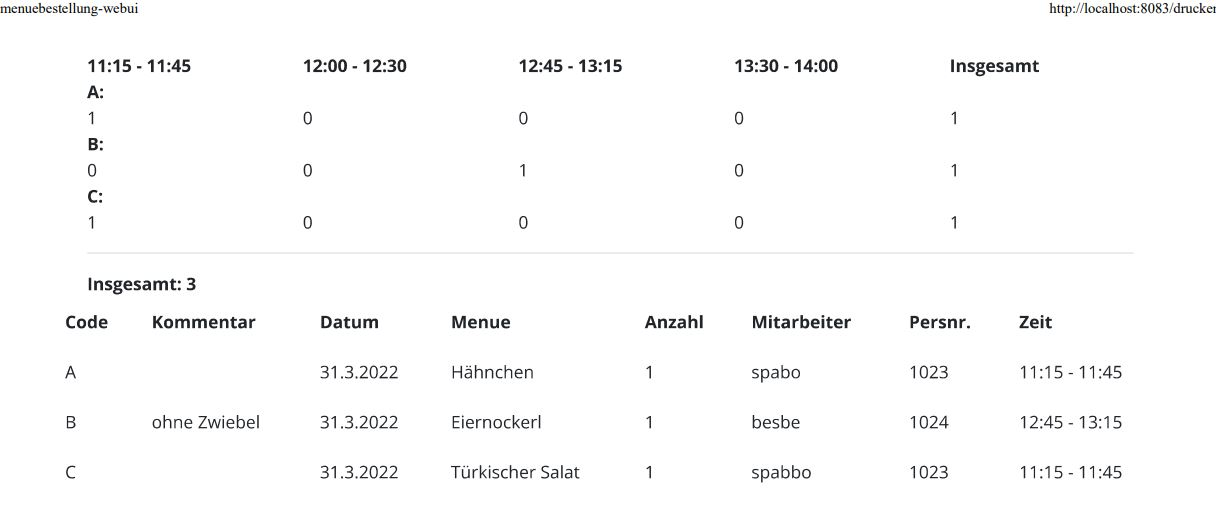
\includegraphics[scale=0.45]{pics/pdf_ansicht.JPG}
    \caption{PDF der Ansicht}
    \label{fig:impl:CantinePrintPDF}
\end{figure}
\pagebreak

\section {Interface Android-App}
\author{Bozidar Spasenovic}


\section{Login}
\begin{figure}[htp]
    \centering
    \author{Bozidar Spasenovic}
    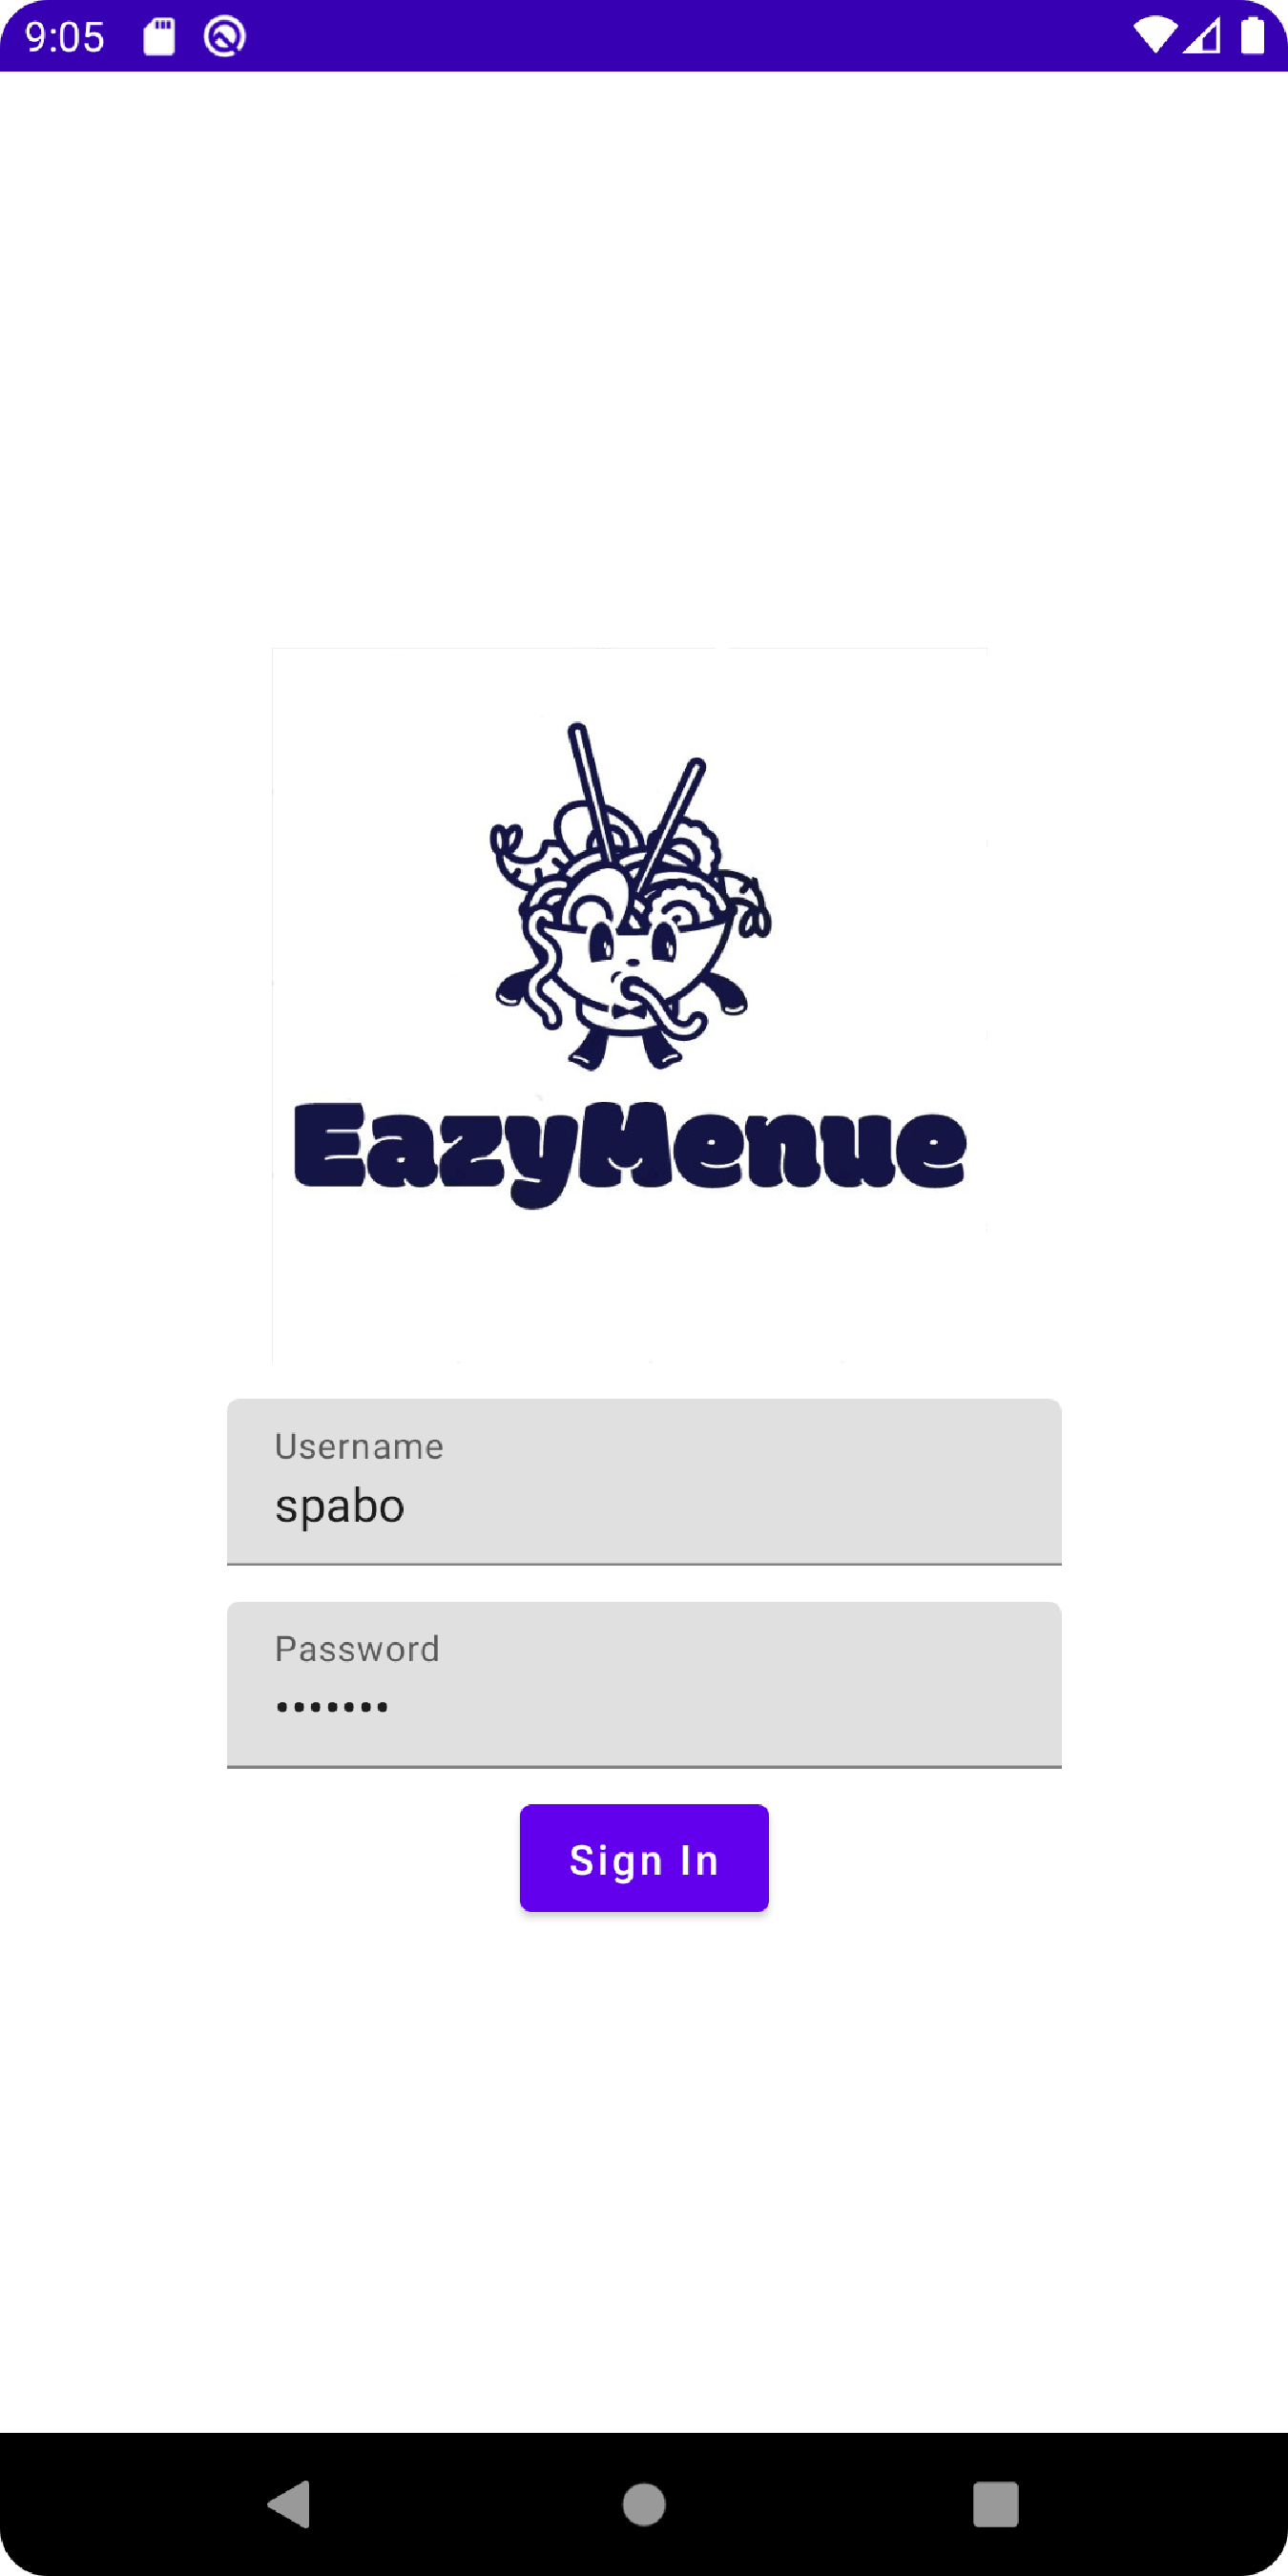
\includegraphics[scale=0.1]{pics/LoginScreenAnndroid.png}
    \caption{Loginscreen Android}
    \label{fig:impl:LoginScreenAnndroid}
\end{figure}

\subsection{Authentification}
Die Authentifizierung erfolgt mit der Methode checkAccessToken, welche nichts anderes macht wie den Keycloak nach einem Token für den User zu fragen.
Kriegt man einen Token zurück, so besteht der User.

\begin{lstlisting}

    Button(onClick = {
        if (!name.isEmpty() && !password.isEmpty() && checkAccessToken()) {

            InitMenues()
            InitBestellungen(name)
            Toast.makeText(
                context,
                "Logged in successfully",
                Toast.LENGTH_SHORT
            ).show()
            isLoggedIn.value = true
            navController.navigate("uebersicht")

        }
    }) {
        Text(text = "Sign In")
    }

\end{lstlisting}

\subsubsection{checkAccessToken()}

Man schickt einen Request an http://10.0.2.2:8082/auth/realms/menuRealm/protocol/openid-connect/token mit einem passendem body.
Im body stehen die Felder die für den Request nötig sind wie zum Beispiel:
\begin{itemize}
    \item die Client ID
    \item der Grant Type 
    \item der Client Secret
    \item der Scope
    \item das Passwort
    \item der Username
\end{itemize}

Als Client wird ein OkHttpClient verwendet. Dieser erstellt einen neuen Aufruf mit dem erstelltem Request. 
Er wartet auf einen Response und speichert bei einem erfolgreichem Response den Token. Da es zu Internet Problemen kommen kann haben wir
einen countDownLatch eingebaut, der vor der Rückgabe der Methode darauf wartet, dass der Token gespeichert worden ist.  

\begin{lstlisting}
    client.newCall(request).enqueue(object : Callback {
        override fun onResponse(call: Call, response: Response) {
            response.use {
                if (response.isSuccessful) {
                    accessToken.value = response.body!!.string()
                }
                else{
                    throw IOException("Unexpected code $response")
                }
            }
            countDownLatch.countDown()
        }
        override fun onFailure(call: Call, e: IOException) {
            e.printStackTrace()
            countDownLatch.countDown()

        }
    })
    countDownLatch.await()
    return accessToken.value != ""
\end{lstlisting}

\subsection{Log out}
Der Mitarbeiter hat eine Möglichkeit sich auch aus der App auszuloggen. Das erfolgt durch den Sign out Button.
\begin{figure}[htp]
    \centering
    \author{Bozidar Spasenovic}
    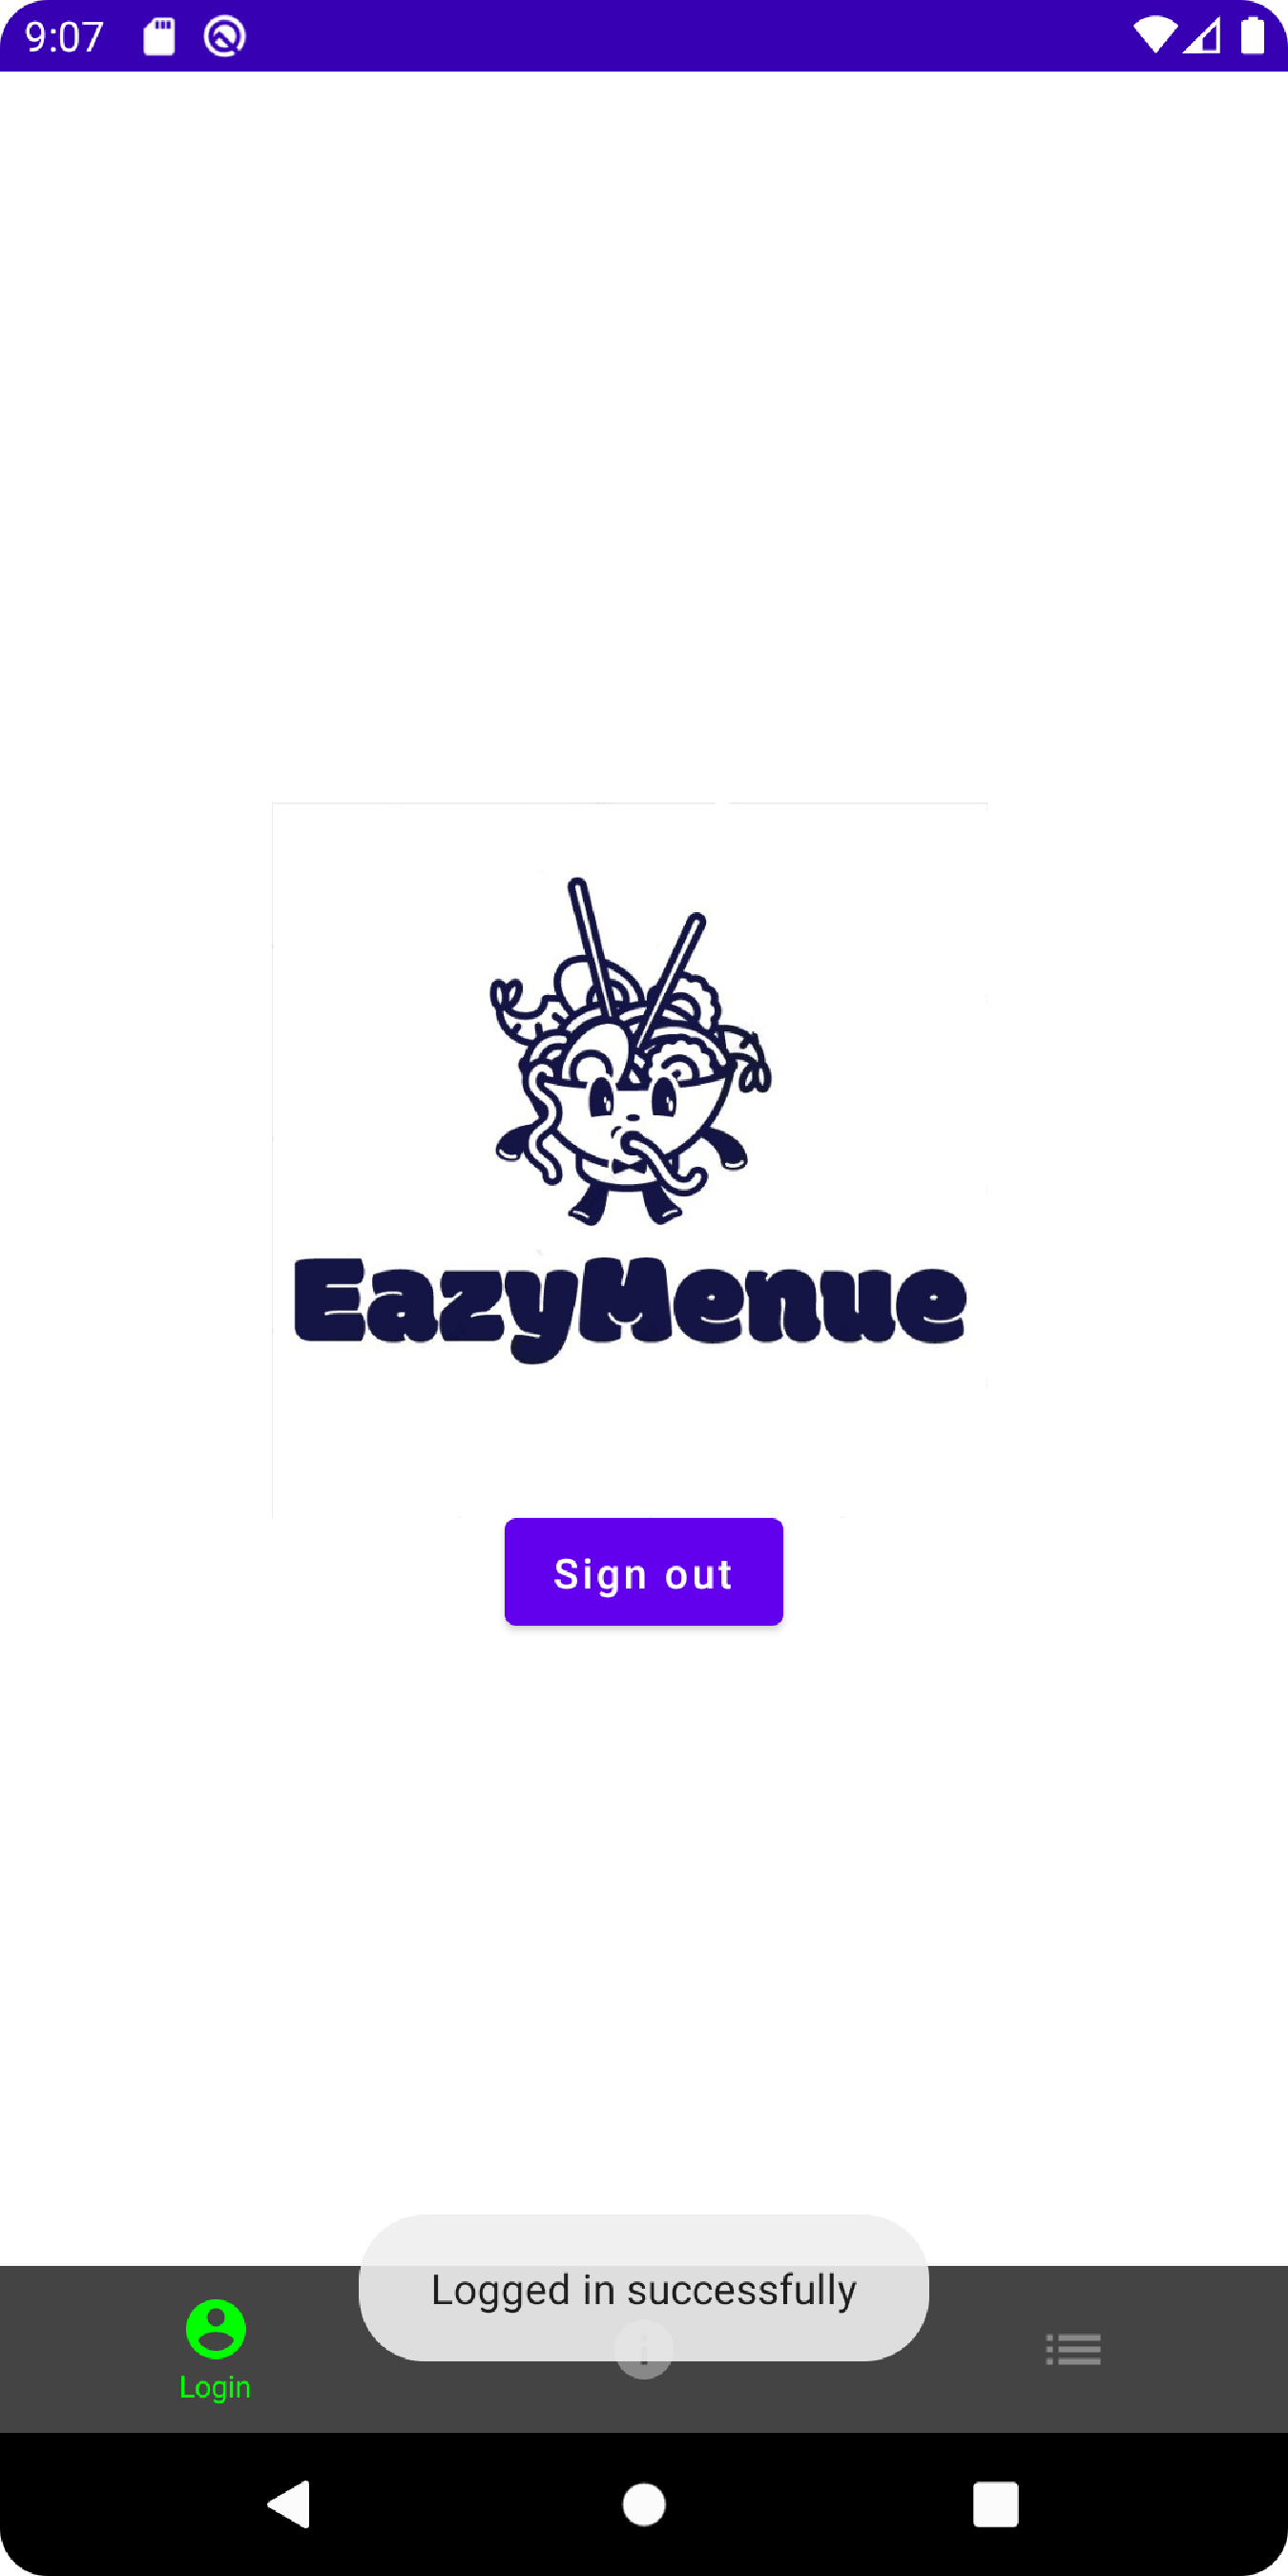
\includegraphics[scale=0.09]{pics/SignOutScreenAnndroid.png}
    \caption{Signout Android}
    \label{fig:impl:SignOutScreenAnndroid}
\end{figure}

Nach dem einloggen wird die Methode InitBestellungen() aufgerufen. Ihre Aufgabe ist es den derzeitigen Bestellungsverlauf des Mitarbeiters zu initialisieren.
Den kann man dann auch in der Verlaufsansicht sehen. 




\pagebreak

\section{Verlauf}

Der Verlauf ist eine einfache Liste von den ganzen Bestellungen des Users.
Es wird der Menüname, das Bestelldatum und das Datum des Menüs angezeigt.
Ist die Bestellung stornierbar, so wird eine Mülltonne als Icon angezeigt. 
Durchs draufklicken auf die Mülltonne, wird die Bestellung storniert.

\begin{figure}[htp]
    \centering
    \author{Bozidar Spasenovic}
    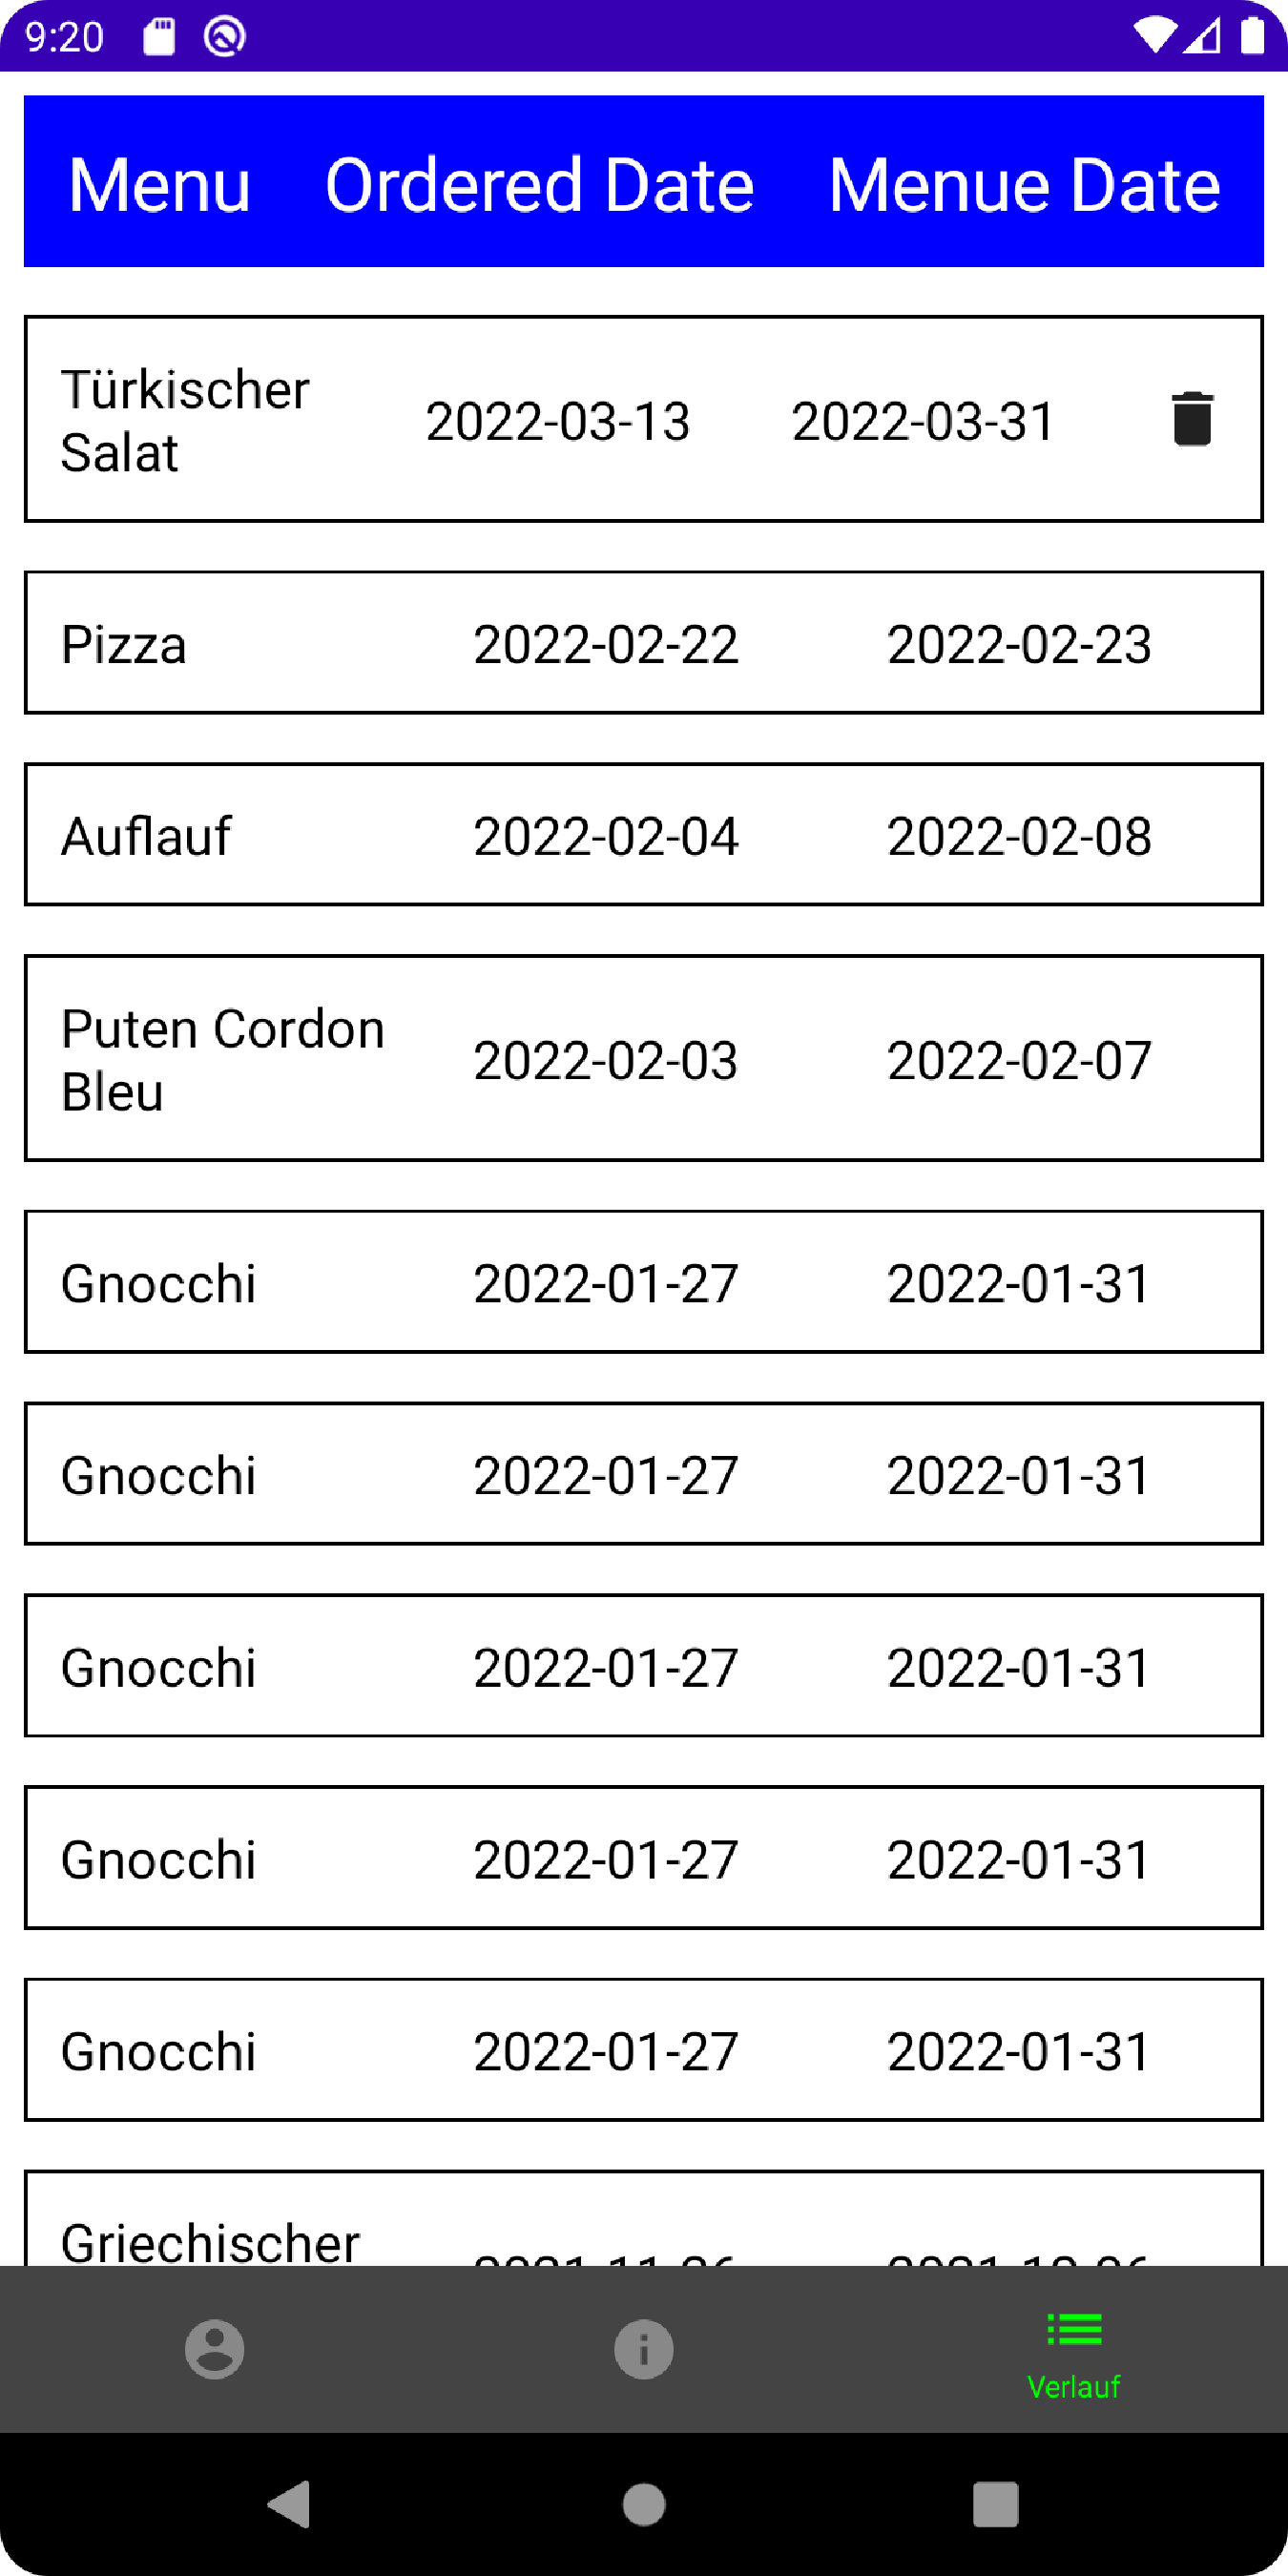
\includegraphics[scale=0.09]{pics/VerlaufAndroid.png}
    \caption{VerlaufAndroid Android}
    \label{fig:impl:VerlaufAndroid}
\end{figure}


Es wird ein PUT auf die URL http://10.0.2.2:8080/menue/bestellung?id=\$menuId was im backend das löschen zur jeweiligen Menü Id ausübt.
Falls ein erfolgreicher Response zurückkommt, so wird die InitBestellungen()-Methode zum neu laden des Verlaufes aufgerufen.

\begin{lstlisting}
    client.newCall(request).enqueue(object : Callback {
        override fun onFailure(call: Call, e: IOException) {
            e.printStackTrace()
        }

        override fun onResponse(call: Call, response: Response) {
            response.use {
                if (!response.isSuccessful){
                    throw IOException("Unexpected code $response")
                }

                InitBestellungen(currUser.value)
            }
        }
    })
\end{lstlisting}


\pagebreak


\section{Bestellansicht}

In der Bestellansicht werden die Felder Menü, Von und das Datum automatisch in ein Readonly Text Field gespeichert.
Man kann dann die Anzahl angeben, für wen man es bestellen möchte und auch zwischen vier Zeiten aussuchen. 

\begin{figure}[htp]
    \centering
    \author{Bozidar Spasenovic}
    \includegraphics[scale=0.09]{pics/BestellübersichtAndroid.png}
    \caption{Bestellansicht Android}
    \label{fig:impl:BestellübersichtAndroid}
\end{figure}

\subsection{postBestellung()}
Nach dem Abschließen wird die postBestellung()-Methode aufgerufen. Sie erstellt einen Requestbody mit den eingegebenen Werten
und schickt es mittels POST an die "http://10.0.2.2:8080/menue/bestellung/" URL. Dieser Endpoint führt dann die Anfrage durch und schickt einen Response zurück.
Wichtig dabei ist es den richtigen Media-Type zu definieren. 

Die Anfrage und Antwort:
\begin{lstlisting}
    client.newCall(request).enqueue(object : Callback {
        override fun onFailure(call: Call, e: IOException) {
            e.printStackTrace()
        }

        override fun onResponse(call: Call, response: Response) {
            response.use {
                if (!response.isSuccessful) throw IOException("Unexpected code $response")

                val gson = GsonBuilder().create()

                val collectionType: Type =
                    object : TypeToken<Collection<Bestellung?>?>() {}.type
                bestellungen = gson.fromJson(response.body!!.string(), collectionType)
            }
        }
    })
\end{lstlisting}

Der Response wird so benutzt, dass man als erstes mit dem GsonBuilder ein Gson-Objekt erstellt.
Dieses Objekt wird verwendet um ein JSON-Objekt in ein Kotlin-Objekt umzuwandeln. 
Damit man Gson verwendetn kann, benötigt man die abhängigkeit com.google.code.gson:gson:2.8.9.
abschliesend wird vom Responsebody eine Collection von allen mitgegebenen Bestellungen erstellt und gespeichert.


